\documentclass[12pt, a4paper]{report}

\usepackage[utf8]{inputenc}
\usepackage[english]{babel}
\usepackage{setspace,enumerate}
\usepackage{amsmath,amssymb,amsthm,mathtools,cases,bm}

\theoremstyle{definition}
\newtheorem{Example}{Example}
\newtheorem{Theorem}{Theorem}

\usepackage{varioref,hyperref,cleveref}
\usepackage[pdftex]{graphicx}
\usepackage{caption,float,epstopdf,subfig}

\renewcommand{\thefigure}{\arabic{figure}}

\usepackage{listings}
\usepackage[dvipsnames]{xcolor}

\lstset{
	language=[ISO]C++,
	backgroundcolor = \color{blue!5!white},
	aboveskip=10pt, belowskip=10pt,
	numbers=left, numberstyle=\tiny,
	tabsize=2,
	breaklines=true,
	basicstyle=\footnotesize\ttfamily,
	keywordstyle = \color{blue!50!cyan}\bfseries,
	commentstyle = \color{darkgray!90},
	stringstyle = \color{OliveGreen},
	morecomment=[l][\color{violet!90!black}]{\#},
	identifierstyle=\color{blue!25!black}
}


\lstdefinelanguage{FreeFem++}[]{C++}{
	morekeywords={int, border, t, pi, label, x, y, sin, cos, pi, mesh, buildmesh, fespace, P1, cout, endl, real, P2, plot, fill, value, cmm, wait, func, macro, solve, solver, CG, int2d, sqrt}
	basicstyle=\footnotesize\ttfamily,
	keywordstyle = \color{blue!25!black},
	stringstyle = \color{blue!25!black}
}
	

\renewcommand*{\thefootnote}{\fnsymbol{footnote}} 
	
\title{\textbf{Deep Learning for PDEs}\\
			\large Report of the joint APSC-NAPDE courses project}
\author{Paolo Joseph Baioni\footnote{\href{mailto:paolojoseph.baioni@mail.polimi.it}{paolojoseph.baioni@mail.polimi.it}}}
\date{\today}

\begin{document}

	
\maketitle

\renewcommand*{\thefootnote}{\arabic{footnote}}
\setcounter{footnote}{0}

	
%%%%%%%%%%%%%%%%%%%%%%%%%%%%%%%%%%%%%%%%%%%%%%%%%%%%%%%%%%%%%%%%%%%%%%%%
%%%%%%%%%%%%%%%%%%%%%%%%%%%%%%%%%%%%%%%%%%%%%%%%%%%%%%%%%%%%%%%%%%%%%%%%	
	

%\chapter*{Acknowledgements}


%%%%%%%%%%%%%%%%%%%%%%%%%%%%%%%%%%%%%%%%%%%%%%%%%%%%%%%%%%%%%%%%%%%%%%%%
%%%%%%%%%%%%%%%%%%%%%%%%%%%%%%%%%%%%%%%%%%%%%%%%%%%%%%%%%%%%%%%%%%%%%%%%
	
\tableofcontents
\clearpage
	
%%%%%%%%%%%%%%%%%%%%%%%%%%%%%%%%%%%%%%%%%%%%%%%%%%%%%%%%%%%%%%%%%%%%%%%%
%%%%%%%%%%%%%%%%%%%%%%%%%%%%%%%%%%%%%%%%%%%%%%%%%%%%%%%%%%%%%%%%%%%%%%%%

\chapter*{Introduction}\label{introduction}
\addcontentsline{toc}{chapter}{Introduction}

The numerical solution of partial derivative equations (PDEs) plays a fundamental role in applied mathematics, science and engineering. \\
The recent advances in machine learning (ML) and the successes obtained by the application of these techniques in various areas suggest the possibility of using ML in solving PDEs. This approach has considerable potential compared to other numerical methods, for example it makes feasible to write mesh-free algorithms, however the theory is not yet developed and consequently important results of convergence and stability are missing, as well as general rules that would allow to identify the optimal parameters for the design of numerical codes. Finally, some intrinsic characteristics of the method make it considerable as a  tool which is complementary to traditional numerical methods, finding application in the field of real-time control. \\
The aim of this project is to get into deep learning techniques and study their  possible applications to PDEs, also reporting some useful theoretical results, as a complement to the methods illustrated during the NAPDE course, and to implement from scratch a Numerical Analysis relevant Neural Networks based C++ program, so to both gain and verify a low-level, detailed and complete understanding of the method and to experiment on some of the programming techniques that have been deepened during the APSC and \textit{``Strumenti di sviluppo e distribuzione di software per la ricerca scientifica''} courses held at PoliMi.\\
The structure of the report is as follows.\\
In chapter \ref{chapter1} we present the general architecture of a Deep Neural Network (DNN) and the main idea of functioning of the algorithm that allows it to learn from the data (Deep Learning), consisting of two phases, called \textit{forward propagation} and \textit{backward propagation}. Therefore, some  sector-specific issues are considered in detail, such as: distinction between train, development and test sets, problems related to overfitting, possible regularization techniques aimed at reducing it, different optimization algorithms and an overview of the main parameters that must be tuned adequately to get good results.\\
In chapter \ref{chapter2} two possible approaches to solving PDEs via DNNs are exposed, also highlighting some choices that can be made in the formulation of the problem and in the treatment of the boundary conditions. We then deepen the comparison between DNNs and the piecewise continuous linear function which are used as bases of finite element spaces of order one, in order to provide a greater intuition of the reasons why the DNN-based method works and to identify, albeit in this particular case, some indications on the ideal number of nodes and layers of the DNN.\\
In chapter \ref{chapter3} we explain the programming architectural choices that have been taken during the development of the code and we illustrate its structure and some of the content of its main files, also providing some insights with respect to the actual implementation of the previously stated theory and methods. The chapter ends with proposing and discussing possible extensions which might be taken in consideration for future developments of the code.\\
Chapter \ref{chapter4} provides instructions on how to obtain,\footnote{The code is freely available on GitHub: \href{https://github.com/pjbaioni/neural-net}{\emph{https://github.com/pjbaioni/neural-net}}} compile, link and run the program, as well as a complete benchmark case, which may be used as test example to verify the correct functioning of the code. After that we dwell on some insights on the behavior of the neural network with respect to those changes in the settings which could be of greater interest, and we illustrate a general procedure for tuning by hand the learning algorithm.\\
In \hyperref[appendix]{appendix} we report the \cite{freefem++} code written for the computations performed in section \ref{section2.2}.


%%%%%%%%%%%%%%%%%%%%%%%%%%%%%%%%%%%%%%%%%%%%%%%%%%%%%%%%%%%%%%%%%%%%%%%%
%%%%%%%%%%%%%%%%%%%%%%%%%%%%%%%%%%%%%%%%%%%%%%%%%%%%%%%%%%%%%%%%%%%%%%%%


\chapter{Neural Networks and Deep Learning}\label{chapter1}
In this chapter we give an introduction to an emerging branch of artificial intelligence which is called \textit{Deep Learning}, and we focus in particular to how to build a \textit{Deep Neural Network} (DNN). Despite this introduction being general, not application-focused, it is not intended to be complete: only the tools relevant for the subsequent chapters are here developed.\\
In the section \ref{section1.1} we explain foundations of neural networks, with the aim of showing how to build a simple DNN and how to train it on data.\\
In the section \ref{section1.2} we talk about some, in a certain sense more specific, aspects of constructing a DNN, which in turn really make the difference in making the algorithm effective. Indeed it turns out that in order to build up a DNN which actually performs well it is necessary to consider with care: the tuning of \textit{hyperparameters}, that are the parameters which are not being optimized by the neural network, the problems arising from over/under-fitting of the data and the techniques used to deal with them, which go under the name of \textit{regularization}, as well as different optimization algorithms, which can become very relevant in order to not remain stuck in a local minima.\\
\newpage
\section{Architecture and operation of a Deep Neural Network}\label{section1.1}
The very fundamental unit which compose every neural network is the \textit{node} or \textit{neuron}, that is a structure that takes some input features, performs a specific transformation on them, and gives the output:
\begin{figure}[H]
\centering
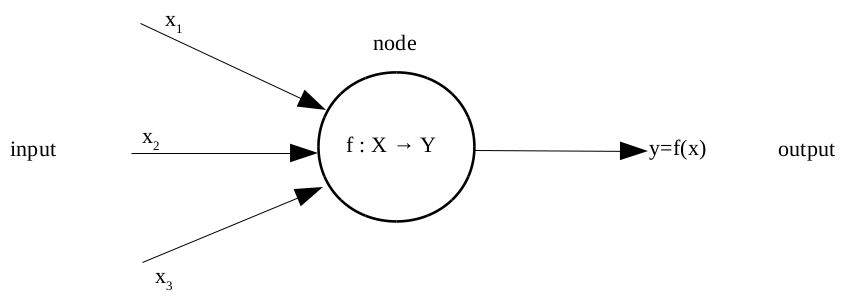
\includegraphics[width=10cm]{img/node}
\caption{Node}\label{fig1}
\end{figure}
\noindent To gain an intuition of what a node is really doing, it's useful to get a more precise idea of a possible problem we could want to face with our node and of an appropriate map $f:X\rightarrow Y$ we might want to use.
\begin{Example}\label{example1}
Consider a given dataset $\{(x_i,y_i)\}$ like the one in the next picture, and suppose to have to find an appropriate relation in the form $y=f(x)$ in order to predict the value of the variable $y$, even for unknown $x$ which we might encounter in the future.
\begin{figure}[H]
	\centering
	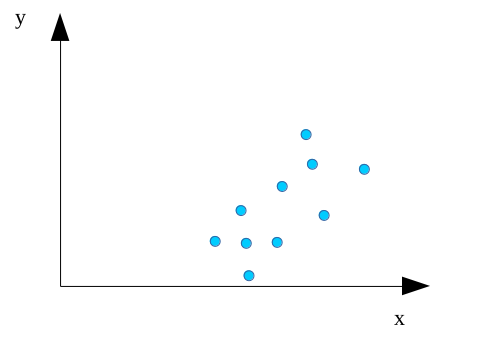
\includegraphics[width=7.5cm]{img/regression1}
	\caption{}
\end{figure}
\noindent As widely known, linear regression can be a first good answer to the problem, so, once performed the calculations, we are able to write:
\[
y=wx + b
\]
for some $w,b$; let's call this linear transformation $L\!: \, Lx=wx+b$. Now suppose that the output $y$ has a constrain, e.g. that $y\ge0$ must hold $ \forall y $.\footnote{The reason why non linear function like the one arising from this constrain are needed in deep learning will be seen in the end of this section.} Then it would be reasonable to update the $f$ function as in the figure below:
\begin{figure}[H]
	\centering
	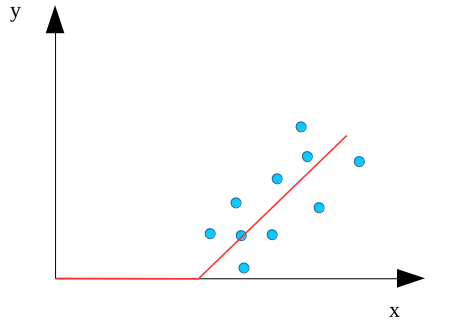
\includegraphics[width=7.5cm]{img/regression2} 
	\caption{}
\end{figure}
\noindent Which mathematically means:
\[
y=max\{0,wx+b\}
\]
So we have that the response function $f$ is given by the composition of a linear function, $L$, and a non linear one, $A\,\,s.t.\,\, x\overset{A}{\longrightarrow}max\{0,x\}$, where of course every function is defined from $X$ to $Y$:
\[
f:X\rightarrow Y\quad s.t.\quad f=A\circ L
\]
In the deep learning literature the non linear function acting after the linear one is called \textit{Activation function}, while the specific one used in this example, namely $x\rightarrow max\{0,x\}$, is known as \textit{ReLU} function, which stands for \textit{Rectified Linear Unit}.$\qed$
\end{Example}
\noindent An approach like the one presented in example \ref{example1} unload all the complexity of a problem on the function $f$ that maps the given data to the predicted output; it thus become early less feasible as complexity grows. It's here that the neural network paradigm come in.\\
The main ideas behind it can be divided in two: a ``divide et impera''-like approach and a statistical-like one, based on random functions and optimization of appropriate functionals.\\
For what concerns the first, the idea is to stuck together different nodes in order to be able to reconstruct complex behaviors as the composition of simpler ones. This assembly of nodes is performed in two fashions: from one side we can imagine to feed in the data to different neurons, which will calculate their own output, and then to put together the outputs, building up what in the literature is called a \textit{layer} of nodes. From the other side we can put different layer in sequence, so that the first layer takes the input from the data, the second layer takes as input the output of the first one, and so on, until the last layer outputs the predicted y.\footnote{Technically it's more correct to say ``every node in the $n\!-\!th$ layer takes the input from every node in the $(n+1)\!-\!th$ layer'', but it's preferred to use the short sentence above when it's clear enough.}\\
Following the literature we call \textit{Hidden layer} every intermediate layer, as in the following picture.
\begin{figure}[H]
\centering
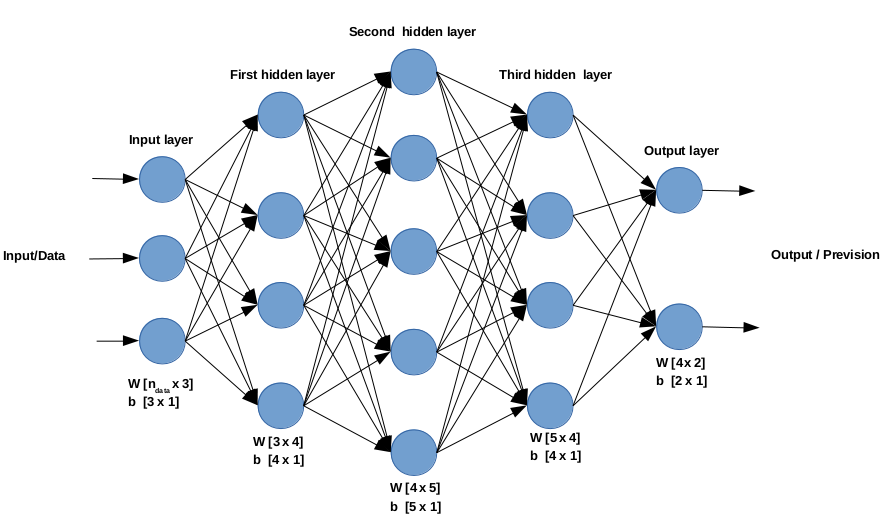
\includegraphics[width=0.95\textwidth]{img/neuralnet}
\caption{Neural network}\label{neuralnet}
\end{figure}
\noindent In deep learning the above mentioned process that brings the input to the output, passing by all the intermediate layers, is called \textit{forward propagation}, or, in short, forprop, and constitute the first part of the training algorithm of a neural network.\\
\newline \noindent One surprising aspect of neural networks is that they don't require their designer to decide which node of the first layer takes which part of the input, nor which nodes of the $n\!-\!th$ layer a generic node of the $(n+1)\!-\!th$ layer should consider, neither how much importance any node should give to each of its inputs. In fact, he gives all the inputs to every node, and lets the neural network find it out by itself. In other words, given enough training samples, i.e. enough $(x_i,y_i)$ known couples, neural networks are remarkably good at figuring out how to map unknown $x$ to the right $y$.\\
This capability is achieved by means of the second main idea of neural networks: what is called \textit{back propagation}, or backprop.\\
Let's consider again the single node as in Figure \ref{fig1}, with $y=ReLU(wx+b)$. More precisely in this case we have:
\begin{equation}\label{linear}
L=\bm{w \cdot x} + b
\end{equation}
where $\bm x = (x_1,x_2,x_3)^T$, $\bm w$ is the vector of the \textit{weights}, since the dot product in \eqref{linear} can be seen as a weighted sum of the inputs, while \textit{b} is called \textit{bias}, since it affects this sum with a its contribution. \\
The basic idea is to perform a forward propagation with known data and randomly initialized parameters $\bm w,b$, then to calculate an appropriate distance between the predicted output, let's call it $\hat y$, and the known output\textit{y}.
This distance measure the \textit{cost C}, or the loss, of our computation.\\
Let's consider for simplicity:
\[
C=\frac{1}{2}(y-\hat y)^2
\]
Now we begin the backprop phase: we calculate the gradient of \textit{C} w.r.t. our parameters, and then we update them using an optimization algorithm aiming at minimizing the cost \textit{C}.\\
For example using gradient descent:
\begin{equation}\label{grad_desc}
\begin{cases}
\bm w \leftarrow \bm w - \alpha \frac{dC}{d\bm w} \\
b \,\,\leftarrow b\,\, - \,\,\alpha \frac{dC}{db}
\end{cases}
\end{equation}
where $\alpha$ is a, typically small, positive real number, which controls how fast we update our weights, and is thus called \textit{learning rate}.\\
The learning process is thus construct as a loop composed by forward propagation followed by backward propagation, with this sequence being repeated until the cost reaches a satisfying value.\\
Coming back to a full DNN, i.e. to a neural network with more than one hidden layer like the one in Figure \ref{neuralnet}, it's easy to generalize the above algorithm.\\
Let's suppose we have a large enough dataset of $x_i$ with the corresponding $y_j$, and divided it in two disjoint subset, the \textit{training set} and the \textit{test set}.\\
We initialize all the weights randomly, and we start the loop, called \textit{training loop}, over the training set.\\
First we have forward propagation:
\begin{itemize}
\item every node of the input layer takes all the data as input, performs an affinity like the one in \eqref{linear} using its own weights and bias, non-linearizes the result through an activation function like the ReLU, and sends it's output to every node of the next layer;
\item every node of the hidden layers takes as input all the outputs coming from the previous layer, performs a weighted sum of them and adds a bias, using its own parameters, and outputs the activated result to each node of the next layer;
\item the nodes in the last layer usually calculate only the linear transformation and outputs the predicted result.\footnote{Unless a binary classification program is being run: in that case it's ok to activate the last layer output too. Further insights will be given later on.}
\end{itemize}
At this point we calculate the value of the cost functional, and then we start backprop, in which every node, starting from the ones inside the last layer, calculate the gradients of the cost w.r.t. its own parameters $w,b$ and updates them using an algorithm like gradient descent. Once we have updated all the parameters till the first layers we do another iteration of the algorithm.\\
When we are satisfied of the performance of our neural network, we do \textit{only one} forward propagation step, keeping the optimal parameters, but using the test set, and we evaluate the accuracy of the results.\\
\newline
\noindent Before going on with the discussion of deeper aspects of deep learning, we show why some of the choices made in the design of the neural network and of the algorithm are appropriate.\\
First of all it is important to notice that non linear activation function are in general necessary. In fact, consider a general DNN, identify with the subscript $l$ the quantities relative to the \textit{l}-th layer, call $n_d$ the number of the data in the set, $n_l$ the number of nodes in the layer l and suppose that $A$ is the identity for each node. We then have:
\[
A_l = L_l = W_l A_{l-1} + b_l
\]
where $A_{l}$ denotes the $n_l \times n_d$ matrix of the outputs of the \textit{l}-th layer, $W_l$ is a $n_{l-1} \times n_l $ matrix, and $b_l$ is a $n_l$ vector. Then we have:
\[
A_l=W_l(W_{l-1}A_{l-2} + b_{l-1})+ b_l = W_lW_{l-1}A_{l-2}+W_lb_{l-1}+b_l =: W'_l A_{l-2} +  b'_l
\]
By recursion is then easy to prove that in the end with a complete step of forward propagation we are computing only a linear combination of the initial data, as we would do in a much simpler way with just one node.\\
In this report we focus mainly on $tanh(\cdot)$ and ReLU activation functions, which are both very common choices, but others are being investigated as well.\\
For similar reasons it is very important to initialize the weights randomly: if we don't, and, for example, we initialize every parameter to a given value, then at the very first iteration all the nodes in the same layer are computing the very same output, and moreover are being updated at the same way during backward propagation. In the end this result in having a DNN that produces the same output of one which has just one node per layer.\\
Finally, it's worth noting that deep neural networks turn out to be more effective than bigger shallow neural networks in reconstructing and predicting complex behavior, especially when it is decomposable in a hierarchical grade of complexity, and that a minimum number of hidden layer is sometimes necessary. We don't prove it, but we will give a quantitative result of a comparison in section \ref{section2.2}, despite in the specific case of reconstruction of continuous piecewise linear functions.


\section{Further insights}\label{section1.2}
When designing a neural network, a great number of choices have to be taken: the number of layers, of nodes, the value of the learning rate, the kind of activation function... Moreover what can be a good setting in one field usually isn't that good in another, making DNN programming a very iterative process. \\
Before getting into it, it's useful to split the data in three sets: the training set, containing the most of the data, the development set and the test set. Then, the first thing to do is to evaluate the performance of the network on the training set: if the error on it is high it means that the network is underfitting the data\footnote{This situation is known in the literature as ``high bias".}, and increasing the size of the network or training it longer could be possible tries. Once the error on the training set is low enough we look at the performance on the dev set. If it is low we've done, otherwise it means that in the previous stage we have overfitted the data\footnote{Also described as a ``high variance" situation.}, that is we have tuned the DNN so much on the training data that it has difficulties to generalize to new ones. In this case we can try to get more data and/ore to use regularization techniques, which are the topic of the next paragraph. It's important to notice that once this modification are done, we've to start again from the beginning and check if the error on the training test is still low enough.\\
Once we have reached a reasonably good result on bot sets, we can finally verify the robustness of our network on the test set, which will give us an unbiased estimation, not having been used yet.\\
This iterative process is resumed in the following flowchart:
\begin{figure}[H]
	\centering
	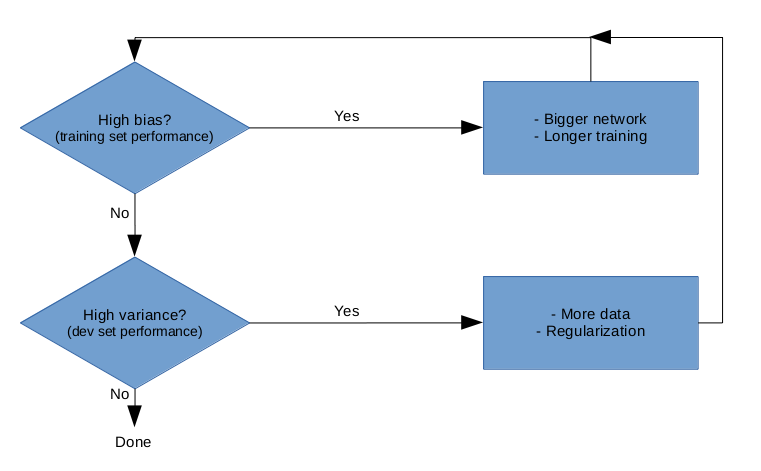
\includegraphics[width=0.9\textwidth]{img/flowchart}
	\caption{}\label{flowchart}
\end{figure}
\noindent Another difficulty comes from the fact that in general the cost functional which has to be minimized is not convex, thus it may have local minima, and the space in which it lives, the one generated by the hyperparameters $W,b$ becomes early high dimensional, enhancing the number of plateaus, and a simple optimization algorithm might stuck in both of them (and it usually do so). Some work can be done on the learning rate and on choice of the optimization algorithm, as it is shown in paragraph \ref{par1.2.2}.\\

\subsection{Regularization}\label{par1.2.1}
There are many kind of regularization techniques, all aiming at reducing the overfitting on the training data. The most common is the $L_2$ \textit{regularization}, which consist in adding a term containing the norms of the parameters to the cost functional:
\[
C \longrightarrow C + \frac{\lambda}{2n_L}\left( \sum_{l=1}^{L}||W_l||_F + ||b_l||_2 \right)^2
\]
where $||\cdot||_F$ indicates the Frobenius norm, $L$ the number of layers and  $\lambda$ the regularization parameter. $L_2$ regularization has the effect of keeping the parameters relatively small, and thus from one side it is somehow as if we had a smaller neural network, and from the other side, being:
\[
A_l=W_lA_{l-1}+b_l
\]
helps keeping the layers more linear, since the activation functions usually have a \textit{tanh}-like form. In both cases $L_2$ regularization force the network to take simpler ``decisions", reducing so the overfitting.\\
Another famous technique is \textit{dropout}, which consist in selecting a different random fraction of the nodes at the beginning of every training iteration, and turning them off by removing the Figure \ref{neuralnet} links. In this way if we look at a single iteration we are working exactly with a smaller network, and so we are reducing overfitting, but at the same time at every iteration we are using a different network, and so we are keeping the capability of the original bigger network to fit the complexity of the data.\\
Of course, while dropout may be useful to find weights able to generalize to data they've never seen, it is meaningful to use it only during the training - development phase of the process, while it hasn't to be used on the test set.

\subsection{Optimization}\label{par1.2.2}
A large number of famous algorithms  in deep learning are based, among the others, on the generalization of the moving averages concept, that is here recalled.\\
Consider a set of data and, for simplicity, figure them as points in a 2D plane; suppose that their pattern follows somehow a certain curve, but in a noisy way. If we want to obtain that smooth curve we can't just take their average, otherwise we'll get a constant line, but we can imagine to cluster them and then to take averages. In order to recover a smooth function, consecutive clusters have to overlap. In practice we can proceed in this way\footnote{We use the notation that we will find when we'll introduce Adam as in \cite{Kingma}. Here $\theta$ is the data. }:
\begin{equation}\label{moving_averages}
\begin{cases}
m_0=0\\
m_t=\beta m_{t-1} + (1-\beta) \theta_t, \quad\quad 0\le\beta\le 1, \, t\geq 1
\end{cases}
\end{equation}
Let's suppose we choose $\beta=0.9$, then roughly speaking \eqref{moving_averages}  computes at every step the average of the last 10 values, producing a quite smooth curve that fits the pattern of the data.\\
\newline \noindent We now introduce four algorithms: gradient descent with momentum, RMS-prop, Adam, which is based on the previous two and that from its presentation at International Conference on Learning Representations in 2015 has became increasingly popular, and its infinity-norm variant AdaMax.\\
\newline \noindent Gradient descent with momentum is the direct application of \eqref{moving_averages} to standard gradient descent. For every iteration t:\footnote{For ease of notation, in the following the $t$ subscript is omitted and the gradient of the objective w.r.t. to a variable it's indicated as d(variable). }
\begin{itemize}\label{momentum}
	\item compute dW, db
	\item update the momenta: 
	\begin{equation}
	\begin{cases}
	m_{dW}\longleftarrow\beta m_{dW} + (1-\beta) dW\\
	m_{db}\longleftarrow\beta m_{db} + (1-\beta) db
	\end{cases}
	\end{equation}
	\item update the parameters:
	\begin{equation}
	\begin{cases}
	W\longleftarrow W - \alpha m_{dW}\\
	b\longleftarrow b - \alpha m_{db}
	\end{cases}
	\end{equation}
\end{itemize}
The effect of the moving averages on gradient descent is a reduction of the oscillations in the path towards the optimum value of $W,b$, which in turn results in a faster convergence: as oscillations go to zero, the whole step is taken in the right direction. In other words, imagine a 2D plane with some parameters that we are optimizing taken as orthogonal axis; then the situation before the addition of the momentum might be portrait as a triangle wave, instead performing averages the vertical oscillations cancels out themselves, while, if the algorithm converges to a point, the displacements to right sum up each other.\\
\newline \noindent RMSprop pursue the same aim, namely fastening convergence of gradient descent when there is an oscillating like behavior, but in a slightly different way:
\begin{itemize}\label{RMSprop}
	\item $\forall t$ compute dW, db
	\item update the momenta: 
	\begin{equation}\label{rms_prop_s}
	\begin{cases}
	s_{dW}\longleftarrow\beta s_{dW} + (1-\beta) dW^2\\
	s_{db}\longleftarrow\beta s_{db} + (1-\beta) db^2
	\end{cases}
	\end{equation}
	\item update the parameters:
	\begin{equation}\label{rms_prop_update}
	\begin{cases}
	W\longleftarrow W - \alpha \frac{dW}{\sqrt{s_{dW}}}\\
	b\longleftarrow b - \alpha \frac{db}{\sqrt{s_{db}}}
	\end{cases}
	\end{equation}
\end{itemize}
where the superscript $2$, indicating square operation, has to be intended element wise, and $s$ stands for square.\\
To visualize the idea behind RMSprop let's suppose to have $dW>>db$; then in every gradient descent iteration it is as if we are taking a great step in the \textit{W} direction, and a significantly smaller one in the $b$ direction. But with RMSprop, if \textit{dW} is big and \textit{db} is small, being $\beta$ usually small, we have in turn $s_{dW}$ big and $s_{db}$ small in \eqref{rms_prop_s}, so in \eqref{rms_prop_update} we take comparable steps in both directions.\\
\newline \noindent As anticipated, Adam basically puts together this two algorithms, and performs a \textit{bias-correction} of the moving averages. The reference for this algorithm is the article by \cite{Kingma}, here we sketch it:
\begin{itemize}\label{Adam}
	\item gradient descent with momentum step:
	\begin{equation*}
	\begin{cases}
	m_{dW}\longleftarrow\beta_1 m_{dW} + (1-\beta_1) dW\\
	m_{db}\longleftarrow\beta_1 m_{db} + (1-\beta_1) db
	\end{cases}
	\end{equation*}
	\item RMSprop step:
	\begin{equation*}
	\begin{cases}
	v_{dW}\longleftarrow\beta_2 v_{dW} + (1-\beta_2) dW^2\\
	v_{db}\longleftarrow\beta_2 v_{db} + (1-\beta_2) db^2
	\end{cases}
	\end{equation*}
	\item momenta correction:
	\begin{equation*}
	\begin{cases}
	m_{dW}^{corr}=\frac{m_{dW}}{1-\beta_1^t},\,\, v_{dW}^{corr}=\frac{v_{dW}}{1-\beta_2^t}\\
	m_{db}^{corr}=\frac{m_{db}}{1-\beta_1^t},\,\, v_{db}^{corr}=\frac{v_{db}}{1-\beta_2^t}
	\end{cases}
	\end{equation*}
	\item parameters update:
	\begin{equation*}
	\begin{cases}
	W\longleftarrow W - \alpha \frac{m_{dW}}{\sqrt{v_{dW}}+\varepsilon}\\
	b\longleftarrow b - \alpha \frac{m_{db}}{\sqrt{v_{db}}+\varepsilon}
	\end{cases}
	\end{equation*}
\end{itemize}
where $\varepsilon$ is a small positive number, used to prevent division by zero.\\
\newline \noindent AdaMax is a variant of Adam, that can be obtained re-formulating the second step by means of the infinity norm. An interesting aspect of this algorithm is that it turns out that doing so we can avoid to correct for initialization bias, as needed in Adam\footnote{See \cite{Kingma}.}. The steps are:
\begin{itemize}\label{AdaMax}
	\item gradient descent with momentum step:
	\begin{equation*}
	\begin{cases}
	m_{dW}\longleftarrow\beta_1 m_{dW} + (1-\beta_1) dW\\
	m_{db}\longleftarrow\beta_1 m_{db} + (1-\beta_1) db
	\end{cases}
	\end{equation*}
	\item infinity norm update:
	\begin{equation*}
	\begin{cases}
	u_{dW}\longleftarrow max\{\beta_2 u_{dW}, |dW| \}\\
	u_{db}\longleftarrow max\{\beta_2 u_{db}, |db| \}
	\end{cases}
	\end{equation*}
	\item parameters update:
	\begin{equation*}
	\begin{cases}
	W\longleftarrow W - \frac{\alpha}{1-\beta_1^t}\cdot \frac{m_{dW}}{\sqrt{u_{dW}}+\varepsilon}\\
	b\longleftarrow b - \frac{\alpha}{1-\beta_1^t}\cdot \frac{m_{db}}{\sqrt{u_{db}}+\varepsilon}
	\end{cases}
	\end{equation*}
\end{itemize}
\noindent \\Before leaving the optimization topic, it's worth mentioning the \textit{learning rate decay}, a technique which involves the progressive reduction of $\alpha$ and that is often used along with the optimization algorithms.\\
Consider for simplicity standard gradient descent. What happens actually is that the steps are quite noisy in the taken direction, not exactly as the previous mentioned triangle wave. This doesn't give big problems at the beginning of the algorithms, but as we approach the minimum we might end up wandering for a technically not finite amount of time about it, but taking too big steps to really reach it. Reducing in an appropriate way the learning rate as the iterations increase in principle doesn't eliminate this problem (unless we exactly hit the minimum), but by sure lead us to wander in a tighter region around the minimum, which usually is a good enough result. Typical choices are:
\begin{itemize}
	\item $\alpha = \frac{1}{1-d*t}\cdot\alpha_0$, \textit{d} being a decay rate,
	\item $\alpha \propto \frac{1}{\sqrt{t}}\cdot\alpha_0$
\end{itemize}
where in both cases \textit{t} stands for the iteration number and $\alpha_0$ is the initial learning rate, but also a simpler piecewise constant decay can make the difference.\\
\newline \noindent In this chapter a significant number of hyperparameters has been explicitly introduced, each of which has to be properly tuned; moreover the list is not exhaustive, for example how to split the data into the three sets has to be decided too\footnote{This depends strongly on the total amount of data, e.g. it could range from $60\%-20\%-20\%$ respectively for train-dev-test sets when we have about $10^3$ data, to $98\%-1\%-1\%$ when we have millions of data, basically because the dev and the test set just have to be big enough to evaluate the performance of the network, while the training set is the one on which the network really \textit{learns} the optimal parameters. Moreover, when having such a big amount of data, it's better considering techniques based on mini-batches.}. Fortunately not all the parameters plays the same role: a good idea might be to start from hyperparameters like the learning rate, the number of hidden units and of nodes per layer, while other parameters like for example the default Adam ones ($\beta_1=0.9,\,\beta_2=0.999,\,\varepsilon=1e-8$) are already good for most applications. 



%%%%%%%%%%%%%%%%%%%%%%%%%%%%%%%%%%%%%%%%%%%%%%%%%%%%%%%%%%%%%%%%%%%%%%%%
%%%%%%%%%%%%%%%%%%%%%%%%%%%%%%%%%%%%%%%%%%%%%%%%%%%%%%%%%%%%%%%%%%%%%%%%


\chapter{Application to PDEs}\label{chapter2}
\setcounter{figure}{5}
The idea of applying machine learning to numerical analysis can be traced back up to \cite{Lagaris}, who tried to solve ODEs and PDEs by means of neural networks. The authors have shown some of the potential of DNNs, such as their being excellent interpolators and the ease of parallelization of the deep learning algorithm; moreover they proposed a first comparison with finite element method and faced the problem one encounters when dealing with boundary value problems (BVPs) in a deep learning setting, which we will expose too. However they still used a mesh, which is a not necessary burden as we'll show, and they used a shallow neural network, with only one hidden layer, that, albeit theoretically able to recover any continuous function, is quite far from being optimal.\\
More recently the explosion of the Big Data field has given rise to stronger interests in deep learning, leading to the development of new tools which are being applied in the study of PDEs too with promising results; for example \cite{Sirignano} face the problem of dimensionality, solving PDEs in space up to 200 dimension using a mesh-free algorithm.\\
Anyway research in this field is still very young, most of the papers having 1-2 years old, and coherently there isn't a solid general theoretical framework as the one of FEM; nonetheless there are already some interesting results, like the one of \cite{Jinchao}.\\
The aim of the present chapter is to outline possible ways of proceeding for problems that one most often encounters in engineering and applied sciences, taking as example the classical Poisson-Dirichlet problem, highlighting pros and cons of the method too (section \ref{section2.1}), and then to provide some useful theorems (section \ref{section2.2}), which compare DNNs accuracy w.r.t. FEMs.
\newpage
\section{The Poisson-Dirichlet problem}\label{section2.1}
There are different ways to employ deep learning to solve the Poisson-Dirichlet problem:
\begin{equation}\label{PoissonDirichlet}
\begin{cases}
-\Delta u = f \quad\quad in\, \Omega\\
u_{|_{\partial\Omega}}=g\qquad on\, \partial\Omega 
\end{cases}
\end{equation}
Recently \cite{Kailai} have obtained good results in few dimension with well-behaved manufactured solutions; their strategy is based on \cite{Lagaris} for the treatment of the boundary condition and on \cite{Sirignano} for the mesh; this method follows.\\
Having in mind what has been said in chapter \ref{chapter1}, the first thing to do is to generate the datasets. Concerning this, there are at least two important things to notice: 
\begin{itemize}
	\item the points can be sampled randomly in $\overline{\Omega}$, so to wipe out the need of a mesh, guaranteeing in this way large computational savings, especially in high dimensions;
	\item the probability that points given by a random generator lie on $\partial \Omega$ is technically zero, since $|\partial\Omega|/|\Omega|=0$, so it has to be ensured that the network is trained on the boundary too.
\end{itemize}
\noindent The authors splits the problem in two similar one, the first having a training set made only by boundary points, the second only by interior points;\footnote{The fundamental aspect is to have ``enough" boundary points. A conceptually simpler solution may be to force the random generator to output an appropriate fraction of boundary points over the total generated, and then to use only one network training on the whole set.} in both cases they use equation \eqref{PoissonDirichlet} RHS to calculate $f,g$ at the random generated points. Then they build up two neural networks, specifically with $3$ layers and $64\times 3$ nodes, $tanh(\cdot)$ activation function and Adam optimizer, to reconstruct the solution $u$ as:
\begin{equation}\label{sol_kailai}
u(x,y;w_1,w_2)=A(x,y;w_1)+B(x,y)\cdot N(x,y;w_2)
\end{equation}
where \textit{A} is the output of the neural network approximating the boundary condition, \textit{N} the one approximating the solution in the domain, and \textit{B} a function that goes to zero on the boundary; consequently their cost functional has the form:
\begin{equation}\label{cost_kailai}
\sum_{i=1}^m\left((g_D)_i - u(x_i,y_i)\right)^2 + \sum_{i=1}^n\left(f(x_i,y_i) - Lu(x_i,y_i)\right)^2
\end{equation}
$L$ being the differential operator in strong form.\\
More precisely their algorithm has two nested loops: for every iteration of the interior network, they perform a full training of the boundary network. Using a $sin(\cdot)sin(\cdot)$ manufactured solution on the unit square with their code, freely available on Github, is possible to recover a very good solution in few hundreds of iterations\footnote{Code and report are here: \cite{Kailai}; notice that it requires \cite{python} 2.7 and \cite{tensorflow}. Figure \ref{pd1} can be found at the same site.}:
\begin{figure}[H]
	\centering
	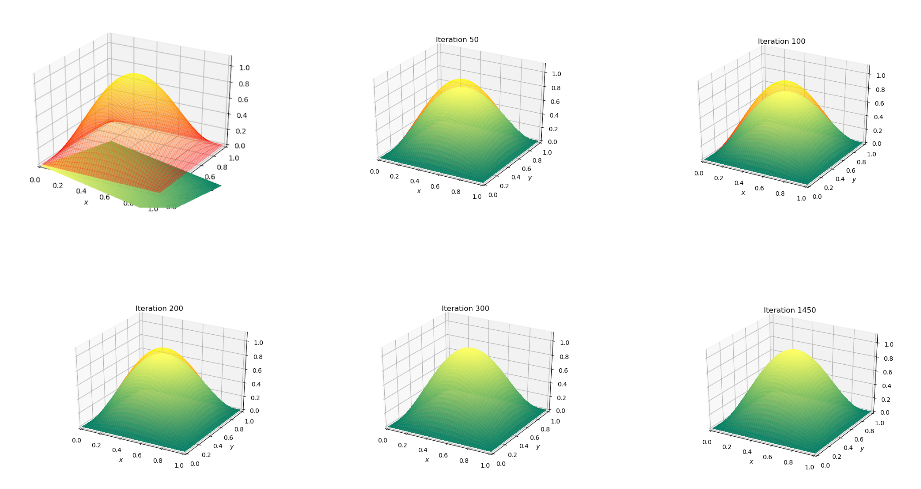
\includegraphics[width=14cm]{img/pd1.png}
	\caption{}\label{pd1}
\end{figure}
\noindent However their algorithm does not perform equally good nor in higher dimension neither with ill-behaved solutions, and further developments are needed.\footnote{Further insights and possible reasons are proposed in the next section.}\\
\newline \noindent A very different approach, but again based on deep learning, has been proposed by \cite{Weinan}. Here it is reported in the case regarding the problem under analysis, in order to show both the largeness of the range of possible DNN based methods for solving PDEs and their common traits, and to point out a very interesting link between this approach, weak formulations and optimal control theory.\\
In their article the homogeneous Poisson-Dirichlet problem is re-casted analytically in the corresponding optimal control problem, leading to a cost functional of the form:
\begin{equation}\label{cost_weinan}
\int_{\Omega}\left(\frac{1}{2} |\nabla u|^2 - uf \right)dx + \beta \int_{\partial\Omega}u^2 d\sigma
\end{equation}
which, besides the positive constant $\beta$ and considering homogeneous Dirichlet conditions, turns out to be the exactly the weak form of the \cite{Kailai} cost functional.\\
The method then proceeds minimizing the cost functional \eqref{cost_weinan} over the set of admissible functions $U_{ad}$, and is here that deep learning comes in. \\
In fact functions in $U_{ad}$ are re-constructed through neural networks, so moving from an additive-like construction proper of standard approximation theory to a compositional-based one.\\
At this point the authors apply a quadrature formula to the integral in \eqref{cost_weinan} and then solve the final optimization problem with a proper optimization algorithm.\\\\
\noindent The algorithm produces good results but, as other approaches based on DNN, has a drawback side: even when the initial problem is convex, the variational problem which is then obtained isn't so, inheriting thus the problem of local minima, plateau and saddle points proper of deep learning.

\section{Some more in-depth theoretical results}\label{section2.2}
In this paragraph some results, obtained mainly by \cite{Jinchao}, are presented, with the aim of giving estimates of the optimal size for a DNN employed to solve PDEs; in particular the results found are useful to ensure that the DNN recovers the same accuracy of the finite element method based on linear base functions.\\
We recall some FEM notation we use in the following: suppose to have a bounded domain\footnote{In the sense of open and connected.} $\Omega\in\mathbb{R}^d$ ad a conforming mesh or grid $\mathcal{T}_h\subset\Omega$, define moreover $k_h$ as the maximum number of mesh elements neighboring a grid point; then the FE space of grade one is:
\[ V_h=\{ v \in C_\Omega \text{ s.t. $v$ is linear on every } \tau_k \in \mathcal T_h \} \]
In other words, the base functions of the grade one FEM are continuous piecewise linear functions, in short CPWL; it is thus natural to proceed into the study using ReLU-DNNs, since the ReLU activation function is a CPWL function and DNNs construct their output as a composition of linear functions and activation functions, giving so a CPWL function as output.\\
\newpage \noindent The two main results are\footnote{These are taken respectively from Theorem 3.1 and Corollary 5.1 of \cite{Jinchao}.}:
\begin{Theorem}\label{thm3.1}
	\textit{Given a locally convex finite element grid $\mathcal T_h$ , any linear finite element function in $\mathbb R^d$ with N degrees of freedom can be written as a ReLU-DNN with at most $\lceil log_2 (k_h)\rceil +1$ hidden layers and at most $\mathcal O(k_hN)$ neurons.}
\end{Theorem}
\begin{Theorem}\label{corol5.1}
	\textit{Given a locally convex finite element grid $\mathcal T_h$ , any linear finite element function in $\mathbb R^d$ with N degrees of freedom can be written as a ReLU-DNN with at most $\lceil log_2 (d+1)\rceil$ hidden layers and at most $\mathcal O(d2^{(d+1)k_h}N)$ neurons.}	
\end{Theorem}
\noindent A direct comparison of the two theorems shows that, although it is possible to achieve linear FEM like accuracy with a relatively shallow network, the deeper one has a considerably smaller size.\\
To fix the ideas it has been considered $d=2$ and $\Omega$ being the unit circle. Then a standard triangulation of the domain is:
\begin{figure}[H]
	\centering
	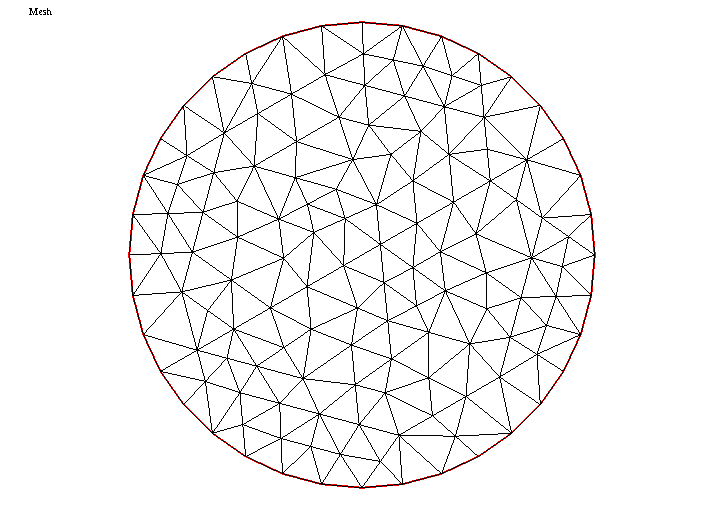
\includegraphics[width=10cm]{img/triangulation.png}
	\caption{Mesh}\label{k_h}
\end{figure}
\noindent When doing an estimate it's thus possible to take $k_h=6$.\\
To find a proper value for N we consider the very well-behaved solution:
\[u_{exact}=e^{-(x^2+y^2)}(x^2+y^2-1)\]
of the problem \eqref{PoissonDirichlet} obtained computing $f$ as $\Delta u_{exact}$; we then solve the problem different times using the FOSS software \cite{freefem++} refining the mesh until a good result is reached.\footnote{Code in \hyperref[appendix]{appendix}.}. \\
We obtain a relative $L_2$ error, defined as $err_{L_2} = \frac{||u_{exact}-u_h||_2}{ \frac{1}{2} (||u_{exact}||_2+||u_h||_2) }  $, of $1.65\%$ when using 36 triangles on the border of the domain, as in Figure \ref{k_h}, which lead to a $V_h$ space with 137 degrees of freedom:
\begin{figure}[H]
	\centering
	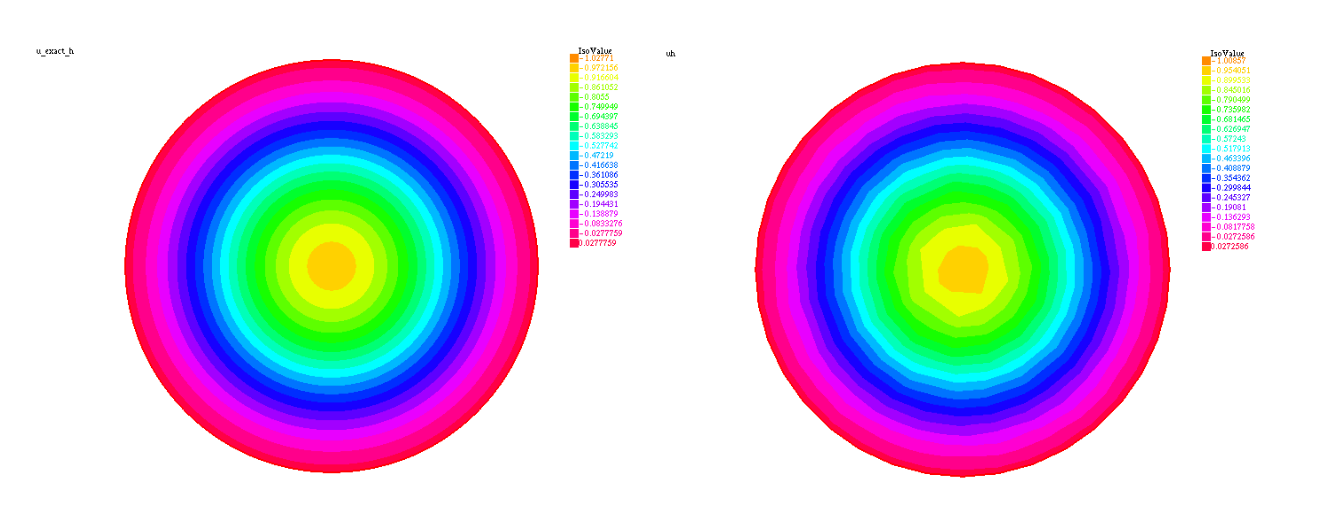
\includegraphics[width=14cm]{img/u2.png}
	\caption{}\label{u2}
\end{figure}
\noindent In the end it is possible to conclude that to recover the same result using a ReLU-DNN \textit{at most}:
\begin{itemize}
	\item $\lceil log_2 (k_h)\rceil +1=4$ layers and $\mathcal O(k_hN)\simeq 10^3$ total nodes, or
	\item $\lceil log_2(d+1) \rceil = 2$ layers and $\mathcal O(d2^{(d+1)k_h}N)\simeq 10^8$ total nodes
\end{itemize}
are needed, confirming that a deep neural network is computational more convenient that a shallow one\footnote{This is coherent with the fact that the power of the neural networks approach stands in their remarkable capability of approximate non linear functions, which is achieved by means of composition between affinities and non linear activation functions, and the step of activation occurs in the forward propagation as many times as the number of layers.} and, perhaps more importantly, giving a quantitative estimate of this convenience.\\


%%%%%%%%%%%%%%%%%%%%%%%%%%%%%%%%%%%%%%%%%%%%%%%%%%%%%%%%%%%%%%%%%%%%%%%%
%%%%%%%%%%%%%%%%%%%%%%%%%%%%%%%%%%%%%%%%%%%%%%%%%%%%%%%%%%%%%%%%%%%%%%%%


\chapter{Implementation of neural-net}\label{chapter3}
\setcounter{figure}{8}
In this chapter an in-depth view of a Deep Learning C++ program, called \textit{neural-net}, is given. As just shown in chapter \ref{chapter2}, what different DNN based PDE solvers have in common is their relying on what turns out to be DNN's numerical analysis strongest point: their remarkably capability of reconstructing function, by means of compositions, which is used to construct the basis of the approximation spaces. For this reason it has been decided to start writing an interpolator based on DNNs; different possible expansions are being investigated as well.\\
The program has been built using the \cite{git} distributed version control system, with GitHub as hosting service, and can be freely cloned or downloaded from the web page: \href{https://github.com/pjbaioni/neural-net}{\emph{https://github.com/pjbaioni/neural-net}}.\footnote{At the moment, already merged branches have not been deleted yet for personal ease in history navigation, e.g. when typing {\ttfamily \$ git log --pretty=format:"\%h \%s" --graph}, but the master branch is the only one which is really active and updated.}\\
In order to build and run the program, some not included dependencies are needed, in particular a C++ compiler, \cite{make}, \cite{gnuplot}, \cite{eigen} and \cite{boost} libraries, while to build the documentation a TeX compiler has to be used; more details are given in the README.md file and in chapter \ref{chapter4}, where it is shown how to obtain, build and run the program. 
\newpage
\section{Directory tree}
Downloading the repository ``neural-net'' one finds:
\begin{itemize}
	\item the \textit{data} folder, which contains the input and output data in .dat and .pot (for \cite{getpot}) format, and \cite{gnuplot} scripts in .gnu format to generate datasets graphs;
	\item the \textit{doc} folder, containing this documentation in .tex and .pdf format, plus the \textit{img} sub-folder where the images included by the TeX file are stored;
	\item the \textit{include} folder, containing the headers \textit{GetPot.hpp}, an utility used for parsing parameters files and command line options, \textit{gnuplot-iostream .hpp}, an utility used to output a graphical representation of the results in an interactive way, \textit{NeuralNetwork.hpp}, which holds the NeuralNetwork class, and \textit{Optimizers.hpp}, where all the optimizers employable from NeuralNetwork are defined as class templates;
	\item the \textit{src} folder, which contain the source files \textit{main.cpp}, \textit{NeuralNetwork.cpp}, where the NeuralNetwork class member functions are defined, the \textit{Makefile} which can be used to automatic build the main program, and the \textit{write\_set} sub-folder, where the \textit{write\_set.cpp} file used to generate datasets is placed;
	\item the COPYING file, a plain text file containing copying informations and licenses;
	\item the README.md file, a markdown file containing basic informations;
	\item the (hidden) \textit{.gitignore} file, that traces the file extensions which are not being pushed to the remote, mainly compilation files, executables and comments file.
\end{itemize}
\noindent Despite their different extensions, every non-png nor non-pdf file can be opened by any text editor.
\section{The Neural Network class}
The class NeuralNetwork implements a computational efficient design of a deep neural network (DNN).\\
As seen in chapter \ref{chapter1}, to which we refer for the names of the principal quantities as for the justification of the main algorithms, a DNN is composed by different layers, each of which is composed by a (possibly) different number of nodes. At the beginning of the present project, this hierarchical structure naturally inherent to DNNs led to the idea of developing three classes, NeuralNetwork, Layer and Node. For reasons that will appear clearer later on\footnote{Basically, because first, internal and last layer performs slightly different works.}, Layer would have been an abstract class, from witch the child classes InputLayer, HiddenLayer and OutputLayer would have inherited. That approach doubtless had the pro of adhering to the abstract model of a DNN, from the more general structure to the really low-level computations, but initial tests have shown that it wasn't so competitive from a computational efficiency point of view, besides being more complex than strictly necessary.\\
The final choice has been to ``vectorize'' the computations as much as possible, grouping together all the operations performed by nodes in each layer by means of matrices.
Of course this passage, which can be considered computationally mandatory in machine learning typical languages such as Python, hasn't brought efficiency by itself, being C++ a compiled language: the difference lies in the fact that it has allowed to rely on strongly optimized well known linear algebra libraries, which have provided considerable computational time savings. In particular the choice is fallen on the \cite{eigen} template library, for its immediate compatibility with C++ and its ease of use and linking with respect to other classical libraries such as Lapack, while maintaining a very good performance.
Having reached this point, and having lost a somehow eye-apparent  sight on each specific node operations, it has appeared senseless to keep the original design of the neural network class, and thus it has been decided to simplify the code, by developing just one class which holds vectors of the quantities that used to characterize every layer in the original design. \\
The choices made have thus led to a structure as the following one:
\begin{lstlisting}[frame=single, name=neuralnet, showstringspaces=false]
class NeuralNetwork{

private:

	//Architecture hyperparameters:
	size_t nlayers;
	VectorXs nnodes;		

	//Parameters to be optimized:
	vector<MatrixXd> W;	
	vector<VectorXd> b;		

	//Forward propagation outputs:
	vector<MatrixXd> L; 	
	vector<MatrixXd> A;		

	//Back propagation gradients:
	vector<MatrixXd> B;		
	vector<MatrixXd> dW;
	vector<VectorXd> db;

	//Optimizers:
	vector<shared_ptr<GradientDescent<MatrixXd>>> W_optimizer;
	vector<shared_ptr<GradientDescent<VectorXd>>> b_optimizer;

public:

	//Constructor:
	NeuralNetwork(const VectorXs &);
	
	//Training function:
	void train(const Eigen::MatrixXd & Data, double alpha, std::size_t niter, const std::size_t W_opt, const std::size_t b_opt, double tolerance=-1., const std::size_t nrefinements=1, const bool verbose=false);
	
	//Test function:
	pair<VectorXd,double> test(const MatrixXd & Data);
	
};

\end{lstlisting}
\noindent Note that here and in most of the following codes all preprocessor's directives as includes and header guards, as well as scope operators, typedefs and comments have been omitted for brevity.\footnote{See NeuralNetwork.hpp for the complete version.}\\
So the class NeuralNetwork holds basically four kind of data members: 
\begin{enumerate}[(i)]
	\item\label{item:i} architecture (hyper)parameters, like {\ttfamily nlayers} and {\ttfamily nnodes}, which specify respectively the total number of layers and the number of nodes for each layer, {\ttfamily VectorXs} being a {\ttfamily typedef} for an Eigen dynamic vector holding {\ttfamily std::size\_t}s, miming the one of {\ttfamily Eigen::VectorXd};
	\item\label{item:ii} the parameters to be optimized, namely {\ttfamily W} and {\ttfamily b}; notice that the latter has to be a vector of vectors, and not a matrix, since the number of nodes varies for each layer;
	\item\label{item:iii} the \textit{propagation members} {\ttfamily L}, {\ttfamily A}, {\ttfamily B}, {\ttfamily dW} and {\ttfamily db}, that hold the data computed at every cycle of forward and backward propagation;
	\item \label{item:iv} the optimizers for {\ttfamily W} and {\ttfamily b}, which hold a (smart) pointer to the base class of the Optimizers class hierarchy.\footnote{Optimizers.hpp is illustrated in section \ref{section3.3}}
\end{enumerate}
For what concerns the (\ref{item:i}) group, {\ttfamily nnodes} is the \textit{true} parameter, indeed it is the only argument that the constructor takes, while {\ttfamily nlayers} is stored for convenience, since it is used very often in for loops in the member functions, but could be removed. In general, it has been chosen to use {\ttfamily std::size\_t} every time an unsigned was needed, to adopt a standard that would fit every necessity.\\
As explained above, {\ttfamily W} and {\ttfamily b} are the vectorized version of chapter \ref{chapter1} parameters: if we call {\ttfamily l} the generic layer, then {\ttfamily W[l]} is an {\ttfamily nnodes(l)}$\times${\ttfamily nnodes(l+1)} matrix, while {\ttfamily b[l]} is a {\ttfamily nnodes(l+1)} column vector, as in Figure \ref{neuralnet}.\\
A similar comment holds for the propagation members (\ref{item:iii}), with two observations:
\begin{itemize}
	\item forward members, {\ttfamily L} and {\ttfamily A}, have been chosen to be the most general possible, even if for the problems for which the program has been designed the first one and the last one will be always column vectors, and not true matrices;
	\item backward members, {\ttfamily B} (which stands for ``backward''), {\ttfamily dW} and {\ttfamily db}, aren't strictly needed, like the previous {\ttfamily nlayers}, but simplify significantly the subsequent code.
\end{itemize}
The (\ref{item:iv}) group has been introduced later, indeed simple algorithms like Gradient Descent can be applied directly during the training phase, i.e. can be written directly by hand in the {\ttfamily training()} function. However it turns out that most finer optimizers need to store estimators of the gradients, and this estimators have to be updated at every training iteration, thus the idea of storing them in the neural net.\\
Since, as it will be seen in the following section, optimizers have been implemented applying inheritance, here we store smart pointers to the base class, instead of the proper optimizer itself, in order to be able to use polymorphism later and to let the user choose the desired optimizer runtime, when calling the training function.\\
\newpage \noindent
Having introduced the data members, we consider now the member functions.\\
The constructor initialize every member, in order of declaration:
\begin{lstlisting}[frame=single, showstringspaces=false]
NeuralNetwork(const VectorXs & nn): nlayers(nn.rows()),nnodes(nn){

	W.reserve(nlayers-1);
	b.reserve(nlayers-1);
	for(size_t l=0; l<nlayers-1; ++l){
		W.emplace_back(MatrixXd::Random(nnodes(l),nnodes(l+1)));	
		b.emplace_back(VectorXd(nnodes(l+1)));
	}

	L.reserve(nlayers);	
	A.reserve(nlayers-1);

	B.reserve(nlayers-1);	
	dW=W; 
	db=b; 

	W_optimizer.reserve(nlayers-1);
	b_optimizer.reserve(nlayers-1);
}
\end{lstlisting}
In all methods whenever possible efficiency has been considered: for example here {\ttfamily nlayers} and {\ttfamily nnodes} are initialized in the member initializer list, and {\ttfamily std::vector<T>::reserve()} followed by {\ttfamily std::vector<T>::emplace\_back()} is preferred over {\ttfamily std::vector<T>::push\_back()}.\\
As already explained {\ttfamily W} has to be initialized randomly; for this purpose it has been chosen to use the Eigen {\ttfamily Random()} function, which returns a double uniformly distributed between zero and one. Of course different choices are possible, for example the ones based on the {\ttfamily <random>} header of the standard library. In particular, to be strictly random, as requested by the chapter \ref{chapter1} argumentation, we should use the latter and guarantee effective randomness including ``real entropy'' in the seed, for example in this way:
\begin{lstlisting}[frame=single, showstringspaces=false]
size_t sd = chrono::system_clock::now().time_since_epoch().count();
default_random_engine gen(sd);
uniform_distribution<double> random_value(0,1);
for(size_t i=0; i<W.rows(); ++i)
	for(size_t j=0; j<W.cols(); ++j)
		W(i,j) = random_value(gen);
\end{lstlisting}
However, the Eigen default pseudo-random function has shown very good performances, so it has been preferred due to its simplicity.\\
It's worth noting that only {\ttfamily W}, {\ttfamily b} and their gradients can be fully initialized, since it has been chosen to take the input data (whatever it is, training or test data, chosen optimizer...) only when it is really used. Consequently variables like the number of data, which is one of the dimension of the {\ttfamily A[l], L[l]} matrices, is not known at this moment.\\
In every case the needed space in the vectors is known from {\ttfamily nlayers}, and thus is pre-allocated; only the strictly needed space is allocated, often only {\ttfamily nlayers-1}, an action that is possible due to the choices made in the following {\ttfamily train()} member function (here decomposed in different frames for clarity):
\begin{lstlisting}[frame=single, showstringspaces=false]
void NeuralNetwork::train(const MatrixXd & Data, double alpha, size_t niter, const size_t W_opt, const size_t b_opt, double tolerance, const size_t nrefinements, const bool verbose){                     
	///////////////////
	//      Init     //
	///////////////////

	size_t ndata=Data.rows();

	//L has nlayers components:
	for(size_t l=0; l<nlayers;++l)
		L.emplace_back(ndata,nnodes(l));
	//A hasn't the last one:
	for(size_t l=0; l<nlayers-1;++l)
		A.emplace_back(ndata,nnodes(l));
	//B hasn't the first one:
	for(size_t l=1; l<nlayers;++l)
		B.emplace_back(ndata,nnodes(l));

	//First layer only reads the input:
	L[0]=Data.col(0); 
	A[0]=L[0];	
\end{lstlisting}
Since the input datasets have to be read somehow, and since the ``layer structure'' was already ready, the first layer has been reserved for reading only. This is of course a personal choice, motivated basically from the fact that it's easy and works good. A more elaborate one could have been to let the first layer weight the $(x,y)$ couples received during training from the dataset, and thus having e.g. {\ttfamily W[0]} an {\ttfamily ndata x nnodes[0]} matrix, but, being {\ttfamily ndata} quite large, this introduces by sure some overhead, which would be unjustified in this case.\\
Since in the present version the first layer only reads the input, it don't need weights, biases and gradients at all, and for this reason their vectors have one component less.\\
A different discussion must be made with regards to the activated outputs variable {\ttfamily A}, which again has just {\ttfamily nlayers-1} elements, but for another reason, less subjective: since we want our output to be a function, in the sense of mathematical analysis, with no particular requirements, we cannot in general activate the last output, because if we would do so for example with a $tanh(\cdot)$, we would be able to reconstruct only $tanh(\cdot)$s.\\
The ``Init'' phase of the {\ttfamily train()} function finishes with the initialization of the optimizers, which is made through a switch-case construct:
\begin{lstlisting}[frame=single]
//Optimizers:
string W_opt_name, b_opt_name;
switch(W_opt){
	case 0:
		for(size_t l=0; l<nlayers-1; ++l)
			W_optimizer.emplace_back(make_shared<GradientDescent<MatrixXd>>(dW[l].rows(),dW[l].cols()));
		W_opt_name = "GradientDescent";
		break;
	case 1:
		for(size_t l=0; l<nlayers-1; ++l)
			W_optimizer.emplace_back(make_shared<GDwithMomentum<MatrixXd>>(dW[l].rows(),dW[l].cols()));
		W_opt_name = "GDwithMomentum";
		break;
	case 2:
		for(size_t l=0; l<nlayers-1; ++l)
			W_optimizer.emplace_back(make_shared<RMSprop<MatrixXd>>(dW[l].rows(),dW[l].cols()));
		W_opt_name = "RMSprop";
		break;
	case 3:
		for(size_t l=0; l<nlayers-1; ++l)
			W_optimizer.emplace_back(make_shared<Adam<MatrixXd>>(dW[l].rows(),dW[l].cols()));
		W_opt_name = "Adam";
		break;
	default:
		for(size_t l=0; l<nlayers-1; ++l)
			W_optimizer.emplace_back(make_shared<AdaMax<MatrixXd>>(dW[l].rows(),dW[l].cols()));
		W_opt_name = "AdaMax";
		break;
}		
	
switch(b_opt){
	case 0:
		for(size_t l=0; l<nlayers-1; ++l)
			b_optimizer.emplace_back(make_shared<GradientDescent<VectorXd>>(db[l].rows(),db[l].cols()));
		b_opt_name = "GradientDescent";
		break;
	case 1:
		for(size_t l=0; l<nlayers-1; ++l)
			b_optimizer.emplace_back(make_shared<GDwithMomentum<VectorXd>>(db[l].rows(),db[l].cols()));
		b_opt_name = "GDwithMomentum";
		break;
	case 2:
		for(size_t l=0; l<nlayers-1; ++l)
			b_optimizer.emplace_back(make_shared<RMSprop<VectorXd>>(db[l].rows(),db[l].cols()));
		b_opt_name = "RMSprop";
		break;
	default:
		for(size_t l=0; l<nlayers-1; ++l)
			b_optimizer.emplace_back(make_shared<Adam<VectorXd>>(db[l].rows(),db[l].cols()));
		b_opt_name = "Adam";
	break;
	case 4:
		for(size_t l=0; l<nlayers-1; ++l)
			b_optimizer.emplace_back(make_shared<AdaMax<VectorXd>>(db[l].rows(),db[l].cols()));
		b_opt_name = "AdaMax";
		break;
}	
\end{lstlisting}
Notwithstanding the possibility to choose different optimizer for {\ttfamily W} and {\ttfamily b} was foreseen only to investigate the relative importance of the two parameters, preliminary tests done trying to predict a wavepacket-like function has shown that the best compromise between accuracy and number of iteration is reached when using AdaMax for {\ttfamily W} and Adam for {\ttfamily b}, so these have become the default.\\
The {\ttfamily train()} function implements a piecewise constant learning rate decay, obtained in this way:
\begin{lstlisting}[frame=single]
///////////////////
//Training loops //
///////////////////
double old_cost{numeric_limits<double>::infinity()};
double cost{-1.}, err{old_cost};
niter=niter/nrefinements;
vector<size_t> backup_t(nrefinements);
	
for(size_t ref=1; ref<=nrefinements; ++ref){
	for(size_t t=1; t<=niter; ++t){
		//do one forward propagation
		//eventually output the cost
		//do one backprop
	}
//update refinement parameters for the next training loop:
alpha=alpha/10;
tolerance=tolerance/((10-2*ref)*10);
} 
\end{lstlisting} 
Learning rate decay has been implemented because it turned out to be very important to obtain acceptable accuracy. This implementation has the pros of being automatic, very simple and effective enough, but, since everything in DNN programming is very problem dependent and has to be tuned properly case by case, better results can be obtained miming this procedure directly in the main, when training the net. Indeed it is enough to don't pass the number of refinements as argument to turn off the automatic learning rate decay, and then implement it manually with subsequent calls to the training function. Guidelines to do it are presented in chapter \ref{chapter4}.\\
The forward propagation step that takes place in the above inner loop follows the general theory:
\begin{lstlisting}[frame=single]
/////////////////////////
// Forward propagation //
/////////////////////////
for(size_t l=1; l<nlayers-1; ++l){
	//Summing the column vector b (nnodes(l+1)x1) to each 
	//column of A*W (ndataxnnodes(l)*nnodes(l)xnnodes(l+1)):
	L[l] = ( A[l-1]*W[l-1] ).rowwise() + b[l-1].transpose();
	A[l] = tanh( L[l].array() );
}	
//The final output shouldn't be activated, otherwise it will be necessarly a tanh:
L[nlayers-1] = ( A[nlayers-2]*W[nlayers-2] ).rowwise() + b[nlayers-2].transpose();
	
//Computing cost as the L2 distance: (divided by 2, for ease in later differentiation)
cost = .5 * (L[nlayers-1] - Data.col(1)).array().square().matrix().sum();
\end{lstlisting}
As evident, the code strongly relies on the Eigen built-in operations and function; in particular at line 7 and 11 of the above code a Python-like \textit{broadcasting} is implemented. Another great advantage of using Eigen is the ease of switching between matrix like operations, like the products in the same lines of code, to element wise operations, which are the ones invoked with a {\ttfamily .array()}. Moreover, when optimization is activated, e.g. with the {\ttfamily g++ -O3} option, conversions from matrices to array, as well as transpositions and so on, are implemented in such a way that they are costless from a computational point of view.\\
Then a convergence check and, eventually, an output to the standard output is performed:
\begin{lstlisting}[frame=single, showstringspaces=false]
/////////////////////////
//  Convergence check  //
/////////////////////////
//Output the current cost
//and check if convergence is reached:
if( t%100==0 ){
	if(verbose)
		cout<<"t="<<t<<" cost="<<cost<<" W_opt="<<W_opt_name<<" b_opt="<<b_opt_name<<" alpha="<<alpha<<"\n";
	err = abs(old_cost-cost) / ( (cost+old_cost)/2 );
	if(err<tolerance){
		backup_t[nref-1]=t;
		break;
	}
	else
		old_cost = cost;
}
\end{lstlisting}
Just after that the backward propagation phase begins. In the initial stages of the project, the backprop algorithm was designed following strictly the standard theory, with vectors of gradients starting from the right of the net and going to the left, e.g. {\ttfamily dW[0]} held the gradient of the cost functional w.r.t. the weights of the last layer.\footnote{See commit 6432f1d517205f3920ab1b77bf224735fbeec819} That designed showed soon some inconveniences: in the update phase we had e.g. {\ttfamily dW[l]} and {\ttfamily W[l]} referring to different layers, and an ad hoc construction for the gradients was needed too, instead of the simpler {\ttfamily dW=W}; for this reason it has been decided soon to ``overturn'' the backprop section while keeping its natural sequence, simply reverting its for loop condition. That's the final code:
\begin{lstlisting}[frame=single]
	//////////////////////////
	// Backward propagation //
	//////////////////////////
	
	//Compute B as d(cost)/d(output): 
	//(no tanh now because it's the last layer)
	B[nlayers-2] = L[nlayers-1] - Data.col(1);	

	for(size_t l=nlayers-2; l>0; --l){
		//Compute gradient of cost wrt W:
		dW[l] = ( L[l].transpose() )*B[l];
		//Update W:
		//W[l] = W[l] - alpha*dW[l];
		(*W_optimizer[l])(W[l],dW[l],alpha,t);
		//Compute gradient of cost wrt b:
		db[l] = B[l].transpose().rowwise().sum();
		//Update b:
		//b[l] = b[l] - alpha*db[l];
		(*b_optimizer[l])(b[l],db[l],alpha,t);
		//Compute previous B: 
		//(now there is tanh, and dx[tanh(x)]=1-x^2)
		B[l-1] = (1. - (A[l].array().square())) * ( (B[l]* (W[l].transpose()) ).array() );
	}
	//Updating parameters of the first hidden layer:
	dW[0] = ( L[0].transpose() )*B[0];
	W[0] = W[0] - alpha*dW[0];
	db[0] = B[0].transpose().rowwise().sum();
	b[0] = b[0] - alpha*db[0];
}//End of the training loop
\end{lstlisting}
\noindent As can bee seen, {\ttfamily B[l]} is a support variable, that holds the derivative of the cost w.r.t to the output of the layer {\ttfamily l}. This is useful since the gradients of the cost w.r.t the weights and the biases are computed by means of the chain rule:
\begin{equation*}
	\begin{cases}
	B[l] := \frac{dC}{dY[l]}\\ 
	\frac{dC}{dW[l]} = \frac{dC}{dY[l]} \cdot \frac{dY[l]}{dW[l]} \\
	\frac{dC}{db[l]} = \frac{dC}{dY[l]} \cdot \frac{dY[l]}{db[l]} \\
	\end{cases}
\end{equation*} 
with \textit{Y[l]} being equal to $L[l]=A[l-1]\times W[l]+b[l]$ for the last layer and to $A[l]=tanh(L[l])$ for the others.\\
The above code implements exactly this chain rule computations, taking into account that the activation function is a $tanh(\cdot)$, and performs also the subsequent update of the parameters, based on their gradients. At the beginning only gradient descent was implemented, directly into the code; that lines have been kept commented for documentation purposes, since they show what the call to the optimizer roughly speaking does.\footnote{Calling the overloaded call operator isn't very elegant anymore, but it was designed when polymorphism wasn't implemented yet, so one had something like {\ttfamily W\_optimizer[l](W[l],dW[l],alpha,t)}, but then polymorphism required to store pointers in the optimizers vectors. Of course one can always do {\ttfamily W\_optimizer[l]->()(W[l],dW[l],alpha,t)}.}\\
\noindent The training function ends with the refinement and the final output:
\begin{lstlisting}[frame=single, showstringspaces=false]
	//update refinement parameters for the next training loop:
	alpha=alpha/10;
	tolerance=tolerance/((10-2*ref)*10);
	}//End of the refinements loop

	//////////////////////////
	//     Final output     //
	//////////////////////////
	size_t total_iter=0;
	for(const auto & r: backup_t)
		r == 0 ? total_iter += niter : total_iter += r;
	cout<<"Total iterations = "<<total_iter<<"\n"<<"Cost functional on the training set = "<<cost<<endl;

}//End of the train function
\end{lstlisting}
where a range-based for loop is used to compute the total number of iterations, since the counter is reset at every refinement. Of course one could have distinguished the cases with refinements from the ones which haven't, for example so to not defining the vector {\ttfamily backup\_t} when not required, but it has been preferred to not do so, in order to avoid a further decision tree in the code. Differently the last check, based on the conditional operator, is needed: it distinguishes between the case in which the inner training loop ends for having reached convergence from the case in which the maximum number of iterations is hit.\\
\newline \noindent The {\ttfamily test()} function performs just one forward propagation, with two main differences w.r.t. {\ttfamily train()}:
\begin{itemize}
	\item it doesn't store nor data neither intermediate results, since it wouldn't re-use them, to save memory;
	\item it is a non-void function, in part due to the above fact, but mainly because one expects to have an output from the test.
\end{itemize}
\begin{lstlisting}[frame=single]
pair<VectorXd,double> test(const MatrixXd & Data){
	//One forprop as before during training,
	//w/o storing anything but the final result:
	MatrixXd Ltest{Data.col(0)};
	MatrixXd Atest{Ltest};
	for(size_t l=1; l<nlayers-1; ++l){
		Ltest = ( Atest*W[l-1] ).rowwise() + b[l-1].transpose();
		Atest = tanh( Ltest.array() );	
	}
	Ltest = ( Atest*W[nlayers-2] ).rowwise() + b[nlayers-2].transpose();
	
	//Computation of the L2 relative error:
	double numerator=(Data.col(1)-Ltest).norm();
	double denominator=(Data.col(1).norm() + Ltest.norm())/2.;
	
	return make_pair(Ltest, (numerator/denominator) );
}
\end{lstlisting}
One could ask why don't use the members {\ttfamily A, L} anyway, so to don't even have to allocate the two matrices. In principle it could be done actually, but it would require more coding: {\ttfamily A[l], L[l]} have to be resized for every {\ttfamily l}, since in general the numerosity of the training set is different from the one of the tests set; instead the above approach has been preferred in order to keep the code as simple as possible.\\
\newline\noindent Before moving to the optimizers classes, we consider some final remarks.\\
The code can be easily extended to a n-D interpolator with no conceptual effort. The very simplest way to do so would be to equip also the first layer with a {\ttfamily W}\footnote{and a {\ttfamily b}, and so even backprop variables too.}, basically to do a (weighted) average of every input point $\bm x = (x_1,x_2,x_3...x_n)$. Indeed, doing so the second layer would take as input just 1D $x$ points as usual, $x$ being the (weighted) averages of the components. This method includes the already implemented one as a special case with n=1 and {\ttfamily W = Ones(ndata,1)}. Moreover also in this case it would be possible to give different importance even to the single tuples of coordinates too, as it has been proposed before for the 1D case. That would by sure introduce some overhead, so it has to be done only if the results won't be satisfactory enough otherwise. Finally that ``squeezing'' from n-D to 1D could be performed later on, in another layer. This action might have two concurring effects: from one side the computational effort of every training iteration is being increased, but from the other one less iterations might be needed to reach convergence, since the richness of the data is being kept ``alive" longer. \\
These improvements haven't been introduced yet, since they go over the aims of the present project as they are outlined in the \hyperref[introduction]{introduction}. Notwithstanding this, it is worth noting that, especially in DNN programming, the more the code is enriched and exponentially the more tuning is necessary; in fact, not only the new choices must be tested, but also all their combinations with the previous hyper-parameters; so the above modifications, albeit quite simple conceptually, could require a slightly significant time to be implemented in an effective way.

\section{The Optimizers class templates}\label{section3.3}
In the {\ttfamily namespace Optimizers\{...\}}, defined in \textit{Optimizers.hpp}, six classes are defined. Since they have to work either with {\ttfamily W} and {\ttfamily b}, they are defined as class templates. Moreover, in order to be able to use polymorphism, so to let the user choose the desired optimizer runtime, they are all related by inheritance, following this hierarchy:
\begin{figure}[H]
	\centering
	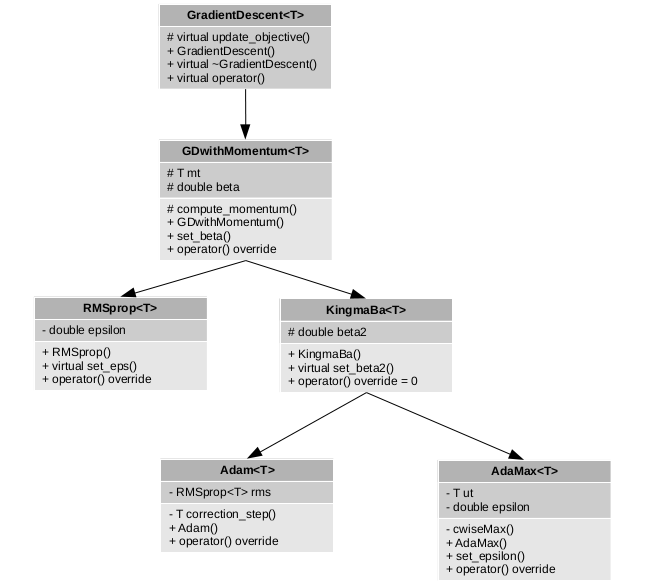
\includegraphics[width=\textwidth]{img/classes1}
	\caption{single inheritance pattern}\label{fig9}
\end{figure}
\newpage \noindent As it was done during early stages of the development, it might seem reasonable to imagine a logical structure like the one sketched here instead:\footnote{``class name = 0'' used as shorthand for ``abstract class''}
\begin{figure}[H]
	\centering
	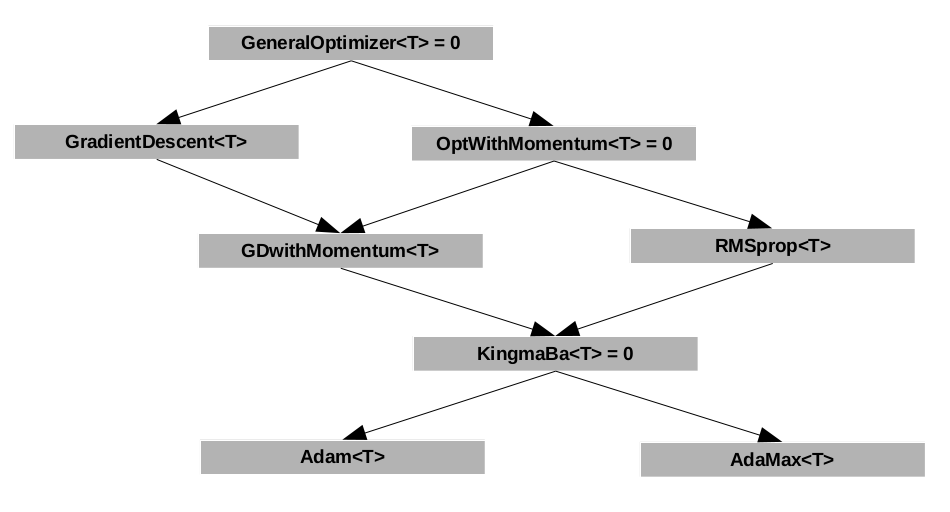
\includegraphics[width=0.9\textwidth]{img/classes2}
	\caption{multiple inheritance pattern}
\end{figure}
\noindent but in this last case the multiple inheritance parts would have involved deadlock diamonds, requiring virtual inheritance.\\
Despite the last one being a possible choice, it has been decided to use only public single inheritance, employing only ``is a'' and ``has a'' relationships, so to keep the code as simple as possible, and also to avoid some overhead.\\
Finally, in order to keep the correct encapsulation even in the single inheritance - Fig. \ref{fig9} design while guaranteeing {\ttfamily Adam<T>} class had the necessary access to the members of its {\ttfamily RMSprop<T>} member {\ttfamily rms}, class {\ttfamily RMSprop<T>} privately declares class {\ttfamily Adam<T>} as friend.\\
\newline \noindent In the following we go a little deeper in some implementation details, class by class.\\
The gradient descent class is straightforward, it's here reported for completeness since it's the base class:
\begin{lstlisting}[frame=single]
template<typename T>
class GradientDescent{
protected:
	virtual void update_objective(T& theta, const T& delta_theta, const double& alpha){
		theta = theta - alpha*delta_theta;  
	}
public:
	GradientDescent()=default;
	GradientDescent(const size_t & m, const size_t & n):GradientDescent(){}
	virtual ~GradientDescent()=default;
	virtual void operator()(T& theta, const T& gt, const double& alpha, const std::size_t & t){
		update_objective(theta,gt,alpha);
	}
};
\end{lstlisting}
\noindent Of course it defines a virtual destructor, even if it doens't do any work more than the default one does, to allow objects in the inheritance hierarchy to be dynamically allocated. Two decisions have been taken, mostly for ease: the template has been kept general, while it could have been specified a little more, using for example {\ttfamily Eigen::MatrixBase<T>}; and unused arguments have been passed to the overloaded call operator, so to have all the arguments that a general optimizer could need, in order to allow overriding in future derived classes.\\
\newline \noindent The gradient descent with momentum class is the first one that implements gradients estimation, for this reason it has a member which is of the same type of the gradient to be estimated:
\begin{lstlisting}[frame=single]
template<typename T>
class GDwithMomentum : public GradientDescent<T>{
protected:
	T mt;
	double beta{0.9};
	virtual void compute_momentum(const T & to_be_averaged){
		mt = beta*mt + (1. - beta)*to_be_averaged;
	}

public:
	GDwithMomentum(const size_t & m, const size_t &n):GradientDescent<T>::GradientDescent(m,n),mt(m,n){}

	virtual void set_beta(double b){beta=b;}

	void operator()(T& theta, const T& gt, const double& alpha, const std::size_t & t) override {
		compute_momentum(gt);
		this->update_objective(theta,mt,alpha);
	}
};
\end{lstlisting}
\newpage \noindent The RMSprop optimizer, besides updating in its own way the objective, it's the first to introduce a member, named epsilon, which is not foreseen in the theory, and that it's here used to prevent division by zero. It's also the first class in the hierarchy to be declared as final, and consequently to use {\ttfamily private} instead of {\ttfamily protected} in its definition: 
\begin{lstlisting}[frame=single]
template<typename T>
class RMSprop final : public GDwithMomentum<T>{
private:
	double epsilon{1e-8};
	friend class Adam<T>;

public:
	RMSprop(const size_t & m, const size_t & n):GDwithMomentum<T>::GDwithMomentum(m,n){}
	virtual void set_eps(double e){epsilon=e;}

	void operator()(T& theta, const T& gt, const double& alpha, const std::size_t & t) override {
		this->compute_momentum(gt.cwiseProduct(gt));
		this->update_objective(theta, (gt.cwiseProduct((1./(epsilon + sqrt(this->mt.array()))).matrix())), alpha);
	}
};
\end{lstlisting}
\noindent Of course, to allow declaring the Adam optimizer as friend class, it has been pre-declared before the definition of {\ttfamily RMSprop<T>}.\\
\newline\noindent The {\ttfamily KingmaBa<T>} class is the only abstract class of the hierarchy. It has been implemented to provide the common interface to two great optimizers, Adam and AdaMax, which have been recently introduced in the same article by \cite{Kingma}:
\begin{lstlisting}[frame=single]
template<typename T>
class KingmaBa : public GDwithMomentum<T>{
protected:
	double beta2{0.999};
public:
	KingmaBa(const size_t & m, const size_t & n):GDwithMomentum<T>::GDwithMomentum(m,n){}
	
	virtual void set_beta2(double b2){ beta2=b2;}

	void operator()(T& theta, const T& gt, const double& alpha, const std::size_t & t)override = 0;
};
\end{lstlisting}
\newpage\noindent The Adam optimizer includes an operation of elevation to the iteration number-th power, which is a non-negative integer. Since {\ttfamily std::pow()} is known to be a ``performance killer", because it solves a non linear problem which is completely unnecessary if the exponent is an integer, at first the {\ttfamily Adam<T>} class employed a function like this one:
\begin{lstlisting}[frame=single, basicstyle=\fontsize{9}{11}\ttfamily]
double mypow(const double b, const std::size_t e){
	double ret{1.};
	for(size_t i=0; i<e; ++i)
		ret*=b;
	return ret;
}

\end{lstlisting}
But later on, compiling with optimization options, it turned out that, at least on the performed test, the standard library function was actually faster, with a total execution time of 4-5 seconds instead of 21-22 seconds on the used machine, and guaranteed a better result too, namely $~2\%$ instead of $~3.9\%$ relative $L_2$ error on the test set.\footnote{This seems to be due to the fact that the iteration number, that is the exponent, becomes early a large number, typical values' order of magnitude ranging from $10^4$ to $10^5$.}\\
So the Adam optimizer has been implemented in this way:
\begin{lstlisting}[frame=single, showstringspaces=false]
template<typename T>
class Adam final : public KingmaBa<T>{
private:
	RMSprop<T> rms;
	T correction_step(const double beta, const std::size_t t, const T & mt){
		return ((1.0/(1.0-std::pow(beta,t)))*mt);
	}
public:
	Adam(const size_t & m, const size_t & n): KingmaBa<T>::KingmaBa(m,n), rms(m,n){}
	void operator()(T& theta, const T& gt, const double& alpha, const std::size_t & t)override{
		//compute the momenta:
		this->compute_momentum(gt);	//GDwithMomentum step
		rms.set_beta(this->beta2);
		rms.compute_momentum(gt.cwiseProduct(gt));//RMSprop step
		//update:
		this->update_objective(theta,( (correction_step(this->beta,t,this->mt)).cwiseProduct( ( 1./(rms.epsilon + sqrt((correction_step(this->beta2,t,rms.mt)).array())) ).matrix() )), alpha);
	}	
};
\end{lstlisting}
The above implementation doesn't strictly follow the one proposed in the literature: the correction step required by the algorithm has been composed with the update step, so to enhance performance. Anyway, also the standard algorithm steps are present in the code, albeit commented out (not reported here to save space).\\
\newline\noindent Last, the AdaMax optimizer:
\begin{lstlisting}[frame=single, showstringspaces=false]
template<typename T>
class AdaMax final : public KingmaBa<T>{
private:
	T ut;
	T cwiseMax(const T& a, const T& b){
		T ret(a.rows(),a.cols());
		if(a.rows()!=b.rows() || a.cols()!=b.cols()){
			std::cerr<<"In AdaMax dimensions must match!\n";
			return ret;
		}
		for(size_t i=0; i<a.rows(); ++i)
			for(size_t j=0; j<a.cols();++j)
				ret(i,j)=std::max(a(i,j),b(i,j));
		return ret;
	}
	double epsilon{1e-8};
	
public:
	AdaMax(const size_t & m, const size_t & n): KingmaBa<T>::KingmaBa(m,n), ut(m,n){}

	void set_epsilon(double e){epsilon=e;}
	
	void operator()(T& theta, const T& gt, const double& alpha, const std::size_t & t)override{
		//compute the momenta:
		this->compute_momentum(gt);		  	//GDwithMomentum step
		ut=cwiseMax(this->beta2*ut,gt.cwiseAbs());//AdaMax step
	
		//update:
		this->update_objective(theta, (( 1. / (1.-std::pow(this->beta,t)) ) * ( this->mt.cwiseProduct( (1./(epsilon+ut.array())).matrix() ) )), alpha);
	}

};
\end{lstlisting}
Notice that the definition epsilon member could have been avoided if multiple inheritance were used.
\newpage
\section{Write\_set and datasets}\label{section3.4}
The src/write\_set folder contains the source file write\_set.cpp, which is used to generate the training and test datasets.\\
This is the first source file to rely to GetPot for the input phase:
\begin{lstlisting}[frame=single, showstringspaces=false]
int main(int argc, char** argv){
	GetPot commandline(argc,argv);
	if(commandline.search(2,"-h","--help")){
		help()<<endl;
		return 0;
	}
	string param_filename = commandline.follow("./../../data/parameters.pot",2,"-p","--parameters");
	GetPot datafile(param_filename.c_str());
	const size_t ntrain = datafile("ntraindata", 70);
	const size_t ntest = datafile("ntestdata", 30);
	VectorXd X;
	X.setLinSpaced(ntrain,-1.5,1.5);
	string file1{"./../../data/TrainingSet"+to_string(ntrain)}, file2{"./../../data/TestSet"+to_string(ntest)};
	write_set(file1+".dat",X);
	X.setLinSpaced(ntest,-1.5,1.5);
	write_set(file2+".dat",X);
	return 0;
}
\end{lstlisting}
The first thing write\_set {\ttfamily main} does is to check the optional parameters passed runtime, if it finds {\ttfamily -h} or {\ttfamily --help} it calls the  help() function, that prints this:\\
{\\\ttfamily \$ ./a.out -h  \\
Run with ./a.out [options]\\
Options:\\
-h, --help: print this help\\
-p, --parameters <filename>: reads parameters from <filename>,\\
          default filename = "./../../data/parameters.pot"\\\\}
and returns; otherwise it reads the number of training and test samples from the parameters file, which can thus be changed without recompiling the program. 
\newpage\noindent The two datasets are then generated calling the following function, which currently generate a wave-packet-like function:
\begin{lstlisting}[frame=single, showstringspaces=false]
constexpr double pi=4.*std::atan(1.);
void write_set(string filename, const VectorXd & X, const char & separator = ' '){
	ofstream ofs(filename);
	auto u = [] (const double & x) {return exp(-x*x*5)*sin(5*pi*x);};	
	for(size_t i=0; i<X.rows(); ++i)
		ofs<<X(i)<<separator<<u(X(i))<<"\n";
	ofs.close();
}
\end{lstlisting}
and are saved in the data folder.\\
To visualize them is possible to use the \cite{gnuplot} script ``PlotDataset.gnu", located in data/ too, eventually modifying the name of the desired dataset. For example for the standard 70 samples training set its output is:\\
{\\ \ttfamily \$ gnuplot PlotDataset.gnu\\
Click any mouse button on selected data point to close}
\begin{figure}[H]
	\centering
	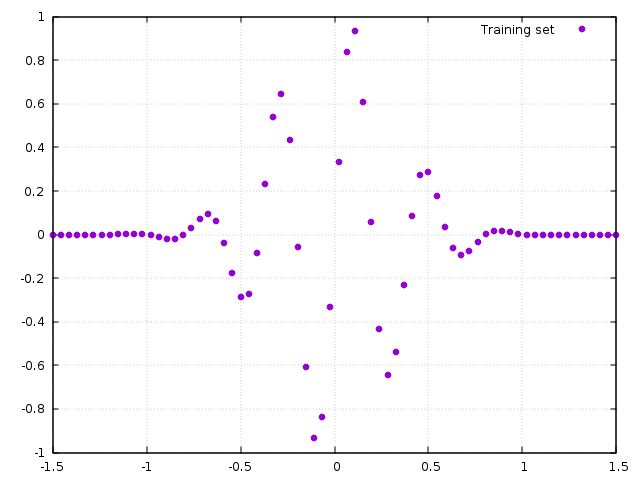
\includegraphics[width=0.95\textwidth]{img/TrainingSet70}
	\caption{70 samples training set}
\end{figure}
\newpage
\section{The main}
The {\ttfamily main.cpp} source file takes into account for both execution of the main program and input/output operations.\\
The input stage is managed analogously to {\ttfamily write\_set.cpp}, thus it's not reported here, for example we have:\\
{\\ \ttfamily 
	\$ ./main.out -h\\
	Run with ./main.out [options]\\
	Options:\\
	-h, --help: print this help\\
	-v, --verbose: activate verbose mode\\
	-p, --parameters <filename>: reads parameters from <filename>,\\
	default filename = "./../data/parameters.pot"\\
	 \\}
So after a first GetPot based input phase, the training dataset and the architecture of the neural network are loaded:
\begin{lstlisting}[frame=single]
//Load the training data:
MatrixXd TrainData(ntraindata,2);
bool read=read_set(train_filename+".dat",TrainData);
if(!read) return -1;

//Load the net architecture:
VectorXs architecture(nlayers);
read=read_set(architecture_filename+".dat",architecture);
if(!read) return -1;
\end{lstlisting}
Since the reading has to work both with matrices and vectors, the read\_set function has been implemented as a function template, so to work with any matrix-like type which implements the overload of the call operator for accessing the elements:
\begin{lstlisting}[frame=single, showstringspaces=false]
template <typename T> 
bool read_set(const string& setname, T & M, const char & separator=' '){

	ifstream in(setname);
	if(!in){
	cerr<<"Error in opening: "<<setname<<std::endl;
	return false;
	}

	string riga,numero;
	for(size_t i=0; getline(in,riga); ++i){
		istringstream rigastream(riga);
		for(size_t j=0;getline(rigastream,numero,separator);++j)
			M(i,j)=stod(numero);
	}
	return true;
}
\end{lstlisting}
After that, the network is constructed following the ``architecture.dat" file instructions, calling the constructor of the NeuralNetwork class, and then trained and tested:
\begin{lstlisting}[frame=single]
//Construct the net:
NeuralNetwork nn(architecture);

//Train the net:
nn.train(TrainData,alpha,niter,W_opt,b_opt,tol,nref,verbose);

//Load the test data:
MatrixXd TestData(ntestdata,2);
read=read_set(test_filename+".dat",TestData);
if(!read) return -1;

//Test the net:
VectorXd yhat;
double errL2;
tie(yhat,errL2)=nn.test(TestData);
\end{lstlisting}
The training results are printed to the standard output by the {\ttfamily train()} function itself, by default only in a synthetic way if the {\ttfamily --verbose} option is not passed to main. \\
Differently, the test results are printed later, directly in the main, both in a written and graphical way. \\
First the numerical results are output on the terminal window and the predicted solution is saved in the prevision file, which by default is data/yhat300.dat:
\begin{lstlisting}[frame=single, showstringspaces=false]
//Print the results:
cout<<"Relative L2 error on test set = "<<errL2<<endl;
write_vector(prevision_filename+".dat",yhat)<<"\n"<<endl;
\end{lstlisting}
by means of the {\ttfamily write\_vector()} function:
\begin{lstlisting}[frame=single, showstringspaces=false]
ostream & write_vector(const string & ofsname, const VectorXd & X){
	ofstream out_file(ofsname);
	streambuf* stream_buffer_cout = cout.rdbuf();
	streambuf* stream_buffer_file = out_file.rdbuf();
	cout.rdbuf(stream_buffer_file);
	cout<<X;
	out_file.close();
	cout.rdbuf(stream_buffer_cout);
	cout<<"Output written on "<<ofsname;
	return cout;
} 
\end{lstlisting}
which redirects the {\ttfamily std::cout} stream buffer to the output file one (and then restore it) to store the y-coordinate only of the predicted function in the file.\\ 
%This steps result in an output like the following:\\
%{\\ \ttfamily 
%	\$ ./main.out\\
%	Total iterations = 16666\\
%	Cost functional on the training set = 0.000157491\\
%	Relative L2 error on test set = 0.00702565\\
%	Output written on ./../data/yhat300.dat\\
%	\\}
In the end, before returning the control to the terminal user, the predicted function is plotted at screen together with the correct solution, given by the test dataset, using the gnuplot-iostream utility:
\begin{lstlisting}[frame=single, showstringspaces=false]
Gnuplot gp;
//first way:
vector<double> xtest(TestData.rows()),ytest(TestData.rows());
VectorXd::Map(&xtest[0], ntestdata) = TestData.col(0);
VectorXd::Map(&ytest[0], ntestdata) = TestData.col(1);
//second way
vector<double> prevision(yhat.data(), yhat.data() + yhat.rows()*yhat.cols());
//plot:
gp<<"plot"<<gp.file1d(std::tie(xtest,ytest))<<
"w lp lw 4 title 'Test Data',"<< gp.file1d(std::tie(xtest,prevision))<<
"w lp lw 1.5 title 'Prevision'"<<endl;
\end{lstlisting}
It's also possible to plot in a second time this last graph without executing again the main program. Indeed, the data folder contains a ``PlotPrevision.gnu" gnuplot script too, which makes use of the {\ttfamily paste}\footnote{ see e.g. {\ttfamily \$ man paste}} GNU coreutil to avoid duplicates of the common x-coordinate:
\begin{lstlisting}[frame=single, showstringspaces=false]
plot "LinspacedTestSet300.dat"	u 1:2 w lp lw 4 title "Test Data", \
"< paste LinspacedTestSet300.dat yhat300.dat" u 1:3 w lp lw 1.5 title "Prevision"
pause mouse "Click any mouse button on selected data point to close\n"
\end{lstlisting}
At the moment of writing, some graphical functionalities, like adding the grid interactively from the plot window, are possible only when the ``PlotPrevision.gnu" script is used, due to current version gnuplot-iostream limitations.


%%%%%%%%%%%%%%%%%%%%%%%%%%%%%%%%%%%%%%%%%%%%%%%%%%%%%%%%%%%%%%%%%%%%%%%%
%%%%%%%%%%%%%%%%%%%%%%%%%%%%%%%%%%%%%%%%%%%%%%%%%%%%%%%%%%%%%%%%%%%%%%%%


\chapter{Examples}\label{chapter4}
\setcounter{figure}{11}
In this chapter we provide a complete example of building and running the program; some info are already reported in README.md.\\
First of all the program can be obtained at \href{https://github.com/pjbaioni/neural-net}{GitHub}. It's suggested to clone the repository, for example if using https executing in a terminal window:\\
{\\ \ttfamily 
	\$ git clone https://github.com/pjbaioni/neural-net\\
\\}
that will create the folder neural-net in the current directory; otherwise, if downloading is preferred, it enough to go \href{https://github.com/pjbaioni/neural-net/archive/master.zip}{here}.\\
In the following it is assumed that the user is in the directory neural-net, that employs the \cite{pacs} course modules, year 2018-2019, and that \cite{eigen} and \cite{boost} modules have been already loaded, e.g. like that:\\
{\\ \ttfamily 
	\$ source /u/sw/etc/bash.bashrc\\
	\$ module load gcc-glibc/7\\
	\$ module load eigen\\
	\$ module load boost\\
	\\}
The program has been tested with the new modules too, in that case of course the second line above should be substituted with:\\
{\\ \ttfamily 
	\$ module load gcc-glibc/9\\
	\\}
Currently the last versions of the code have been tested only with modules, but there should be no problems at all if a local standard installation of the required libraries is used. In this case in the passages that follows the directives that make use of environmental variables starting with {\ttfamily mk} have to be corrected in such a way that they take the path to the correct directories.
\newpage
\section{Building}
The main program is built through \cite{make}; in particular in the src folder this Makefile is placed:
\begin{lstlisting}[frame=single]
CXXFLAGS += -std=c++14 -Ofast #-O3 #-ffast-math
CPPFLAGS += -DNDEBUG -I$$mkEigenInc -I$$mkBoostInc -I./../include/
LDLIBS += -L$$mkBoostLib -lboost_filesystem -lboost_system -lboost_iostreams
OUTPUT_OPTION=-o $@
EXE = main.out
HEADERS=./../include/$(wildcard *.hpp)
SRCS=$(wildcard *.cpp)
OBJS=$(SRCS:%.cpp=%.o)
OPTIONS=#if_empty_minimal_output

main.o: $(HEADERS) $(SRCS)
NeuralNetwork.o: $(HEADERS) $(filter-out main.cpp,$(SRCS))

.PHONY: all build clean distclean run

.DEFAULT_GOAL = build

all: build

build: $(EXE)

$(EXE): $(OBJS)
	$(CXX) $(CXXFLAGS) $(LDLIBS) $^ $(OUTPUT_OPTION)

clean:
	$(RM) $(OBJS)

distclean: clean
	$(RM) $(EXE)

run:
	./$(EXE) $(OPTIONS)
\end{lstlisting}
which, beside defining some useful variables and phony calls, compiles the objects relying on implicit rules, and then links them explicitly.\\
To build the program it's thus sufficient to run the makefile while being in the src folder:\\
{\\ \ttfamily 
	neural-net\$ cd src\\
	src\$ make\\
	\\}
Typing {\ttfamily make all} or {\ttfamily make build} will produce the same result. The expected output is:\\
{\\ \ttfamily 
 src\$ make \\
g++ -std=c++14 -Ofast -DNDEBUG -I\$mkEigenInc -I\$mkBoostInc\\ -I./../include/  -c -o NeuralNetwork.o NeuralNetwork.cpp\\
g++ -std=c++14 -Ofast -DNDEBUG -I\$mkEigenInc -I\$mkBoostInc\\ -I./../include/  -c -o main.o main.cpp\\
g++ -std=c++14 -Ofast -L\$mkBoostLib -lboost\_filesystem\\ -lboost\_system -lboost\_iostreams NeuralNetwork.o main.o -o main.out\\
	\\}
Of course the program can be built even without Make; it's enough to copy and paste the three above instruction to the terminal.\\
\newline\noindent To be run, the program requires some data, examples of which are already provided in the data folder. Input datafiles can be edited in any way, but, for what concerns the training and test datasets, the easiest way is to use the provided {\ttfamily write\_set.cpp} utility.\\
To do build it, while being in the src folder, it's enough to type:\\
{\\ \ttfamily 
	src\$ cd src/write\_set\\
	write\_set\$ g++ -std=c++14 -I\$mkEigenInc -I./../../include/\\ write\_set.cpp\\
\\}
Mind that, since it uses GetPot, if the only changes concern the numerosity of the datasets, after having built it once it's enough to change the ``parameters.pot" file in the data folder. As showed in section \ref{section3.4}: \\
{\\ \ttfamily 
	write\_set\$ ./a.out --help\\
\\}
gives some info more about that.\\
\newline\noindent For what concerns the modifications when modules are not used, for write\_set it's enough to change the line as:\\
{\\ \ttfamily 
	write\_set\$ g++ -std=c++14 -I/path/to/eigen/directory/\\ -I./../../include/ write\_set.cpp\\
\\}
Similar changes, for both the {\ttfamily -I} and the {\ttfamily -L} directives, are required in the Makefile for the main program.
\newpage
\section{Reconstruction of a wave packet}
As first example of execution, the program is run using the provided datasets ``LinspacedTrainingSet70.dat" and ``LinspacedTestSet300.dat", using the architecture provided in ``architecture.dat".\\
Having built the main program as in the previous section, while being in the src folder we tipe:\\
{\\ \ttfamily 
	src\$ make run\\
\\}
which gives:\\
{\\ \ttfamily 
Total iterations = 70300\\
Cost functional on the training set = 0.000127854\\
Relative L2 error on test set = 0.00665947\\
Output written on ./../data/yhat300.dat\\
}
\begin{figure}[H]
	\centering
	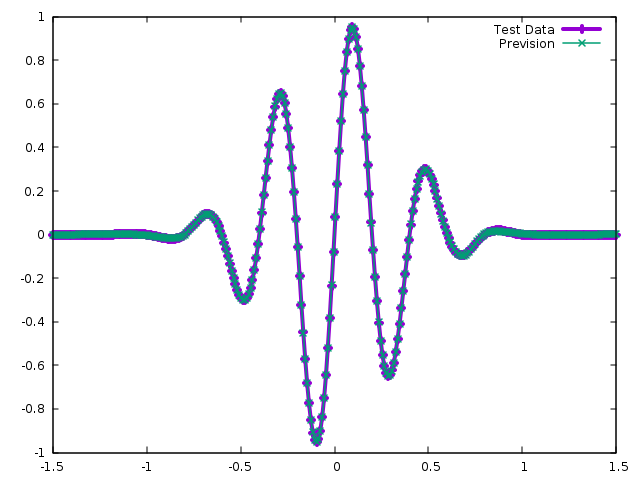
\includegraphics[width=\textwidth]{img/Prevision300} 
	\caption{Test1 - 300 samples}
\end{figure}
\noindent showing very good results. It might be noticed that, as anticipated in chapter \ref{chapter1}, actually the test set has to be just big enough to check the performance of the net. For this purpose the ``LinspacedTestSet30.dat" it's perfect, and indeed its output is:\\
{\\ \ttfamily 
	Total iterations = 70300\\
	Cost functional on the training set = 0.000127854\\
	Relative L2 error on test set = 0.00722058\\
	Output written on ./../data/yhat30.dat\\
\\}
However the 300 samples version has been chosen as standard because the 30 samples test set gives rise to a too low resolution graph:
\begin{figure}[H]
	\centering
	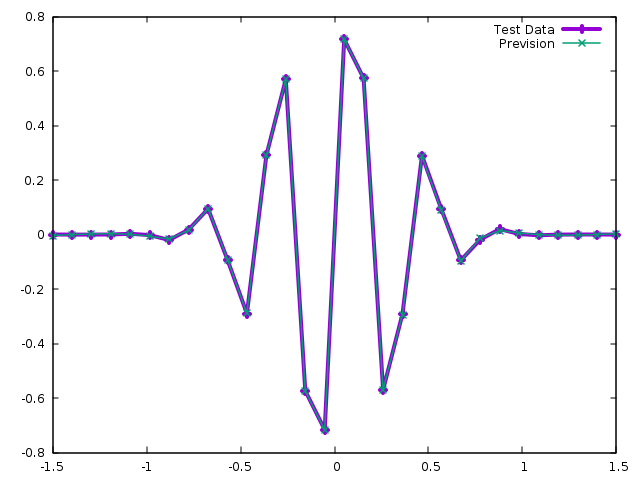
\includegraphics[width=\textwidth]{img/Prevision30} 
	\caption{Test2 - 30 samples}
\end{figure}
\newpage \noindent It's also possible to pass options to the main by make, redefining the variable {\ttfamily OPTIONS} runtime, e.g.:\\
{\\ \ttfamily 
src \$ make run OPTIONS=-p="parameters.pot" OPTIONS+="--verbose"\\
./main.out -p=parameters.pot --verbose\\
t=100 cost=2.14956 W\_opt=AdaMax b\_opt=Adam alpha=0.01\\
t=200 cost=1.43787 W\_opt=AdaMax b\_opt=Adam alpha=0.01\\
t=300 cost=0.996626 W\_opt=AdaMax b\_opt=Adam alpha=0.01\\
...\\
t=24900 cost=0.000127942 W\_opt=AdaMax b\_opt=Adam alpha=0.0001\\
t=25000 cost=0.000127854 W\_opt=AdaMax b\_opt=Adam alpha=0.0001\\
Total iterations = 70300\\
Cost functional on the training set = 0.000127854\\
Relative L2 error on test set = 0.00665947\\
Output written on ./../data/yhat300.dat\\
\\}
Some parameters can be changed editing the ``parameters.pot" file (or another one, and passing it's name to main):
\begin{lstlisting}[frame=single,showstringspaces=false]
###########################################################
######### Runtime data for Neural Network - main ##########
###########################################################

# When tuning the net, it's better to start from alpha and 
# architecture keeping others parameters s.t. the program 
# runs long enough, with nrefinements = 1. 

# Number of training samples:
ntraindata = 70

# Number of test samples:
ntestdata = 30

# Number of layers:
nlayers = 9

# (Initial) learning rate:
alpha = 0.01

# Maximum number of training iterations:
niter = 75000

# (Initial) Tolerance (for convergence check):
tol = 0.001

# Weights optimizer:
# 0 = Gradient descent
# 1 = Gradient descent with momentum
# 2 = RMS prop
# 3 = Adam
# 4 = AdaMax
W_opt = 4

# biases optimizer (values as above):
b_opt = 3

# Number of refinements for alpha decay:
nref = 3
\end{lstlisting}
It's worth noting that increasing the net size not necessarily results in a better performance. For example, if it is used as architecture {\ttfamily \{1, 14, 12, 11, 15, 11, 14, 13, 15, 12, 1\}}, that corresponds to a neural net composed by one reading and ten working layers, the hidden ones with a random number of nodes between 11 and 15, the output on the same dataset is:\\
{\\ \ttfamily 
Total iterations = 75000\\
Cost functional on the training set = 6.82184e-08\\
Relative L2 error on test set = 0.0543924\\
Output written on ./../data/yhat300.dat\\
\\}
meaning that the net is starting to overfit the training data, and thus to have difficulties to generalize to the unseen test data; on the contrary, if we take a more complex function, e.g. one with more oscillations, a deeper and bigger network will be needed to obtain good results.\\
In very extreme underfitting and overfitting case, even NaNs and Infs can be appear, so in general a good procedure is to start with a smaller network, since in this case the result is produced faster, and then to add layers and nodes until the results starts to get worse.\\
\newline\noindent As previously mentioned, it might happen that better results are achieved with an hand made piecewise constant learning rate decay. To do that it's enough to:
\begin{enumerate}
	\item\label{item:1} change the {\ttfamily train(...)} line in main.cpp so that it doesn't take {\ttfamily tol, nref} and {\ttfamily verbose}, and fix a low {\ttfamily alpha}, say $0.01$, and a large {\ttfamily niter}, say 25000;
	\item execute the code, and notice at what iteration the cost starts to become constant or oscillating;
	\item change the {\ttfamily niter} to that number;
	\item add another training line with a lower {\ttfamily alpha}, for example $0.001$, and a large number of iterations, as at point \ref{item:1};
	\item repeat until you get a good result.
\end{enumerate}
Of course, instead of doing as at point \ref{item:1}, parameters can be changed also in parameters.pot; for example point \ref{item:1} it's equivalent to put {\ttfamily nref}=1, {\ttfamily tol}=$-1.0$, {\ttfamily alpha}=0.01, {\ttfamily niter}=25000 and to run the code with the ``{\ttfamily -v}" (or ``{\ttfamily --verbose}") option.\\
As last remark, it's worth underlining that changing the architecture will invalidate the optimality of the {\ttfamily alpha} and {\ttfamily niter} couples of hyper-parameters found following the above procedure.


%%%%%%%%%%%%%%%%%%%%%%%%%%%%%%%%%%%%%%%%%%%%%%%%%%%%%%%%%%%%%%%%%%%%%%%%
%%%%%%%%%%%%%%%%%%%%%%%%%%%%%%%%%%%%%%%%%%%%%%%%%%%%%%%%%%%%%%%%%%%%%%%%


\chapter*{Conclusions}
\addcontentsline{toc}{chapter}{Conclusions}
In the \hyperref[chapter1]{first chapter} of this report we have illustrated in detail the mechanism behind deep learning, going also over the surface for what concerns typical problems one encounters when designing a deep neural network, such as hyperparameter tuning and overfitting, proposing solutions like $L_2$ regularization and dropout and giving an idea of the scheme one can follow when tuning the network. Moreover we've showed how gradient descent can be extended to tackle deep learning problems, till arriving to Adam and AdaMax, which have been proposed the first time in 2015 and which are now employed in many different situations.\\
In chapter \ref{chapter2} we have showed two main techniques which can be used to face PDEs problems by means of deep neural networks, as some interesting and useful theoretical results, following the most recent articles and reporting pros, like the ease of extension to more dimensions, aspects that require some care, like the treatment of BCs, and problems that are still open, in general related to the lack of a theoretical framework, implying among the others uncertainty about theoretical error bounds and appropriate values of hyperparameters.\\
In chapters \ref{chapter3} and \ref{chapter4} we have focused on explaining how a DNN based efficient and numerical analysis relevant application has been developed from scratch, exposing both the technicalities of the adopted algorithms and the design choices that have been taken, both in the details of the implementation and in the general architecture of the program; some insights into expansions of possible interest have been discussed too. After this a complete benchmark case  has been presented, accompanied by comprehensive instructions on how to build and run the program.\\
Before concluding, we notice that it isn't uncommon to find comparisons between results achievable with DNNs methods and classical ones, for example \cite{Jinchao} prove that in a 1D specific example a ReLU DNN can recover a better result, in terms of convergence accuracy, than adaptive finite element method, while \cite{Weinan} show that with fewer parameters, their DNN based method gives more accurate solution than the finite difference method . In such comparisons it's worth considering that the time required by a DNN-like approach is very different from the one of standard methods, indeed from one side tuning a DNN program properly requires a large amount of time, because even hyperparameters which have given great results in one field of application are often completely not suitable to the others, so a considerably high number of combinations have to be tried; from the other side, once tuned and trained, the DNN it's always ready to perform different tests, and so to make all the predictions needed, just at the price of one forward propagation, while a standard solver has to work every time from scratch.\\ 
Considering all these aspect, we can certainly conclude that deep learning is a very promising and interesting field even for numerical analysis, both from the theoretical and from the applications point of view.\\
Moreover, its completely specific time scales makes it particularly adapt to find its natural space in the standard procedure of computational science and engineering: if we have an engineering machine or a scientific experiment on which we have to able to operate in very short times, for example to perform rapid slight changes to the configuration in response to sudden perturbations so to guarantee the stability of the system, we start proceeding with the mathematical modeling of the physical problem, we analyze it theoretically and then we move to numerical analysis and finally to programming for example a FEM code. At this point we can design a DNN based solver which we train on the solutions we have found with the previous methods. In this way we end up with a software which is able to find in very short times, the time of just one forward propagation, solutions to the model when the data, i.e. the physical situation, has changed a little, providing in such a way a powerful tool for the real-time control of the state of the machine or of the experiment.


%%%%%%%%%%%%%%%%%%%%%%%%%%%%%%%%%%%%%%%%%%%%%%%%%%%%%%%%%%%%%%%%%%%%%%%%
%%%%%%%%%%%%%%%%%%%%%%%%%%%%%%%%%%%%%%%%%%%%%%%%%%%%%%%%%%%%%%%%%%%%%%%%


\appendix
\chapter*{Appendix}\label{appendix}
\addcontentsline{toc}{chapter}{Appendix}
The code used in section \ref{section2.2} follows:
\begin{lstlisting}[language=FreeFem++, frame=single, name=extimate_dof, showstringspaces=false]
// Code written to extimate the number of degrees 
// of freedom (dof) needed to reach a good extimate
// in section 2.2 of the report.

///////////////////////////////////
////////////Instructions///////////
///////////////////////////////////

/*	
To run the code, save it as and edp file: <filename>.edp
(Note that edp files can be opened by any text editor, saving
as .txt works as well)
Then in a terminal emulator do:
$ FreeFem++ <filename>.edp

The code has been tested on Debian 9.9,
equipped with FreeFem++ version  3.47 

pjbaioni 2020
*/

///////////////////////////////////
////////////////Code///////////////
///////////////////////////////////

// Mesh
int n=36; 
//n->dofs: 9->13, 12->20, 16->30, 18->41, 20->45, 36->137
border c(t=0, 2*pi){x=cos(t); y=sin(t); label=1;}
mesh Th=buildmesh(c(n));
plot(Th,cmm="Mesh",wait=1);

// Space
fespace Vh(Th,P1);
cout<<"Degrees of freedom N = "<<Vh.ndof<<endl;

// Manufactured solution:
real a=1.;
mesh T=buildmesh(c(5*n));
fespace V(T,P2);
V uexact = exp(-a*(x^2+y^2))*(x^2+y^2-1);
plot(uexact,fill=1,value=1,cmm="u_exact_h",wait=1);

// Data
func f = -4*exp(-a*(x^2 + y^2))*(a^2*x^4 + 2*a^2*x^2*y^2 - a^2*x^2 + a^2*y^4 - a^2*y^2 - 3*a*x^2 - 3*a*y^2 + a + 1);
func g = 0;

// Solution
Vh uh,vh;
macro grad(u) [dx(u), dy(u)] //
solve poisson2d(uh,vh,solver=CG)=int2d(Th)(grad(uh)'*grad(vh))//'
-int2d(Th)(f*vh)
+on(1,uh=g);
plot(uh,fill=1,value=1,cmm="uh",wait=1);

//L2 error (normalized)
real num=int2d(Th)((uexact-uh)*(uexact-uh)); num=sqrt(num);
real den1=int2d(Th)(uexact*uexact); den1=sqrt(den1);
real den2=int2d(Th)(uh*uh); den2=sqrt(den2);
real den=(den1+den2)/2;
cout<<"Relative error in  L2 norm = "<<num/den<<endl;

// Expected output:
/*
  --  mesh:  Nb of Triangles =    236, Nb of Vertices 137
Degrees of freedom N = 137
--  mesh:  Nb of Triangles =   5706, Nb of Vertices 2944
-- Solve : 
min -0.981309  max -1.42832e-31
Relative error in  L2 norm = 0.0165159
times: compile 0.016902s, execution 0.093685s,  mpirank:0
CodeAlloc : nb ptr  2902,  size :366776 mpirank: 0
Ok: Normal End
*/

\end{lstlisting}



%%%%%%%%%%%%%%%%%%%%%%%%%%%%%%%%%%%%%%%%%%%%%%%%%%%%%%%%%%%%%%%%%%%%%%%%
%%%%%%%%%%%%%%%%%%%%%%%%%%%%%%%%%%%%%%%%%%%%%%%%%%%%%%%%%%%%%%%%%%%%%%%%


\newpage
\begin{thebibliography}{10}
	\addcontentsline{toc}{chapter}{Bibliography}
	
	\bibitem[APSC]{pacs} Advanced Programming for Scientific Computing course lectures and material, Politecnico di Milano, 2019.
	\bibitem[Andrew NG]{AndrewNG} Professor Andrew NG's Deep Learning MOOC at Coursera, \href{https://www.coursera.org/specializations/deep-learning}{\emph{https://www.coursera.org/specializations/deep-learning}}, consulted in 2019.
	\bibitem[Boost]{boost} Boost C++ libraries, \href{https://www.boost.org/}{\emph{https://www.boost.org/}}
	\bibitem[cppreference.com]{cppreference} An online reference of the C++ language, \href{https://en.cppreference.com/w/cpp}{\emph{https://en.cppreference.com/w/cpp}}
	\bibitem[Eigen]{eigen} Eigen C++ template library for linear algebra, \href{https://eigen.tuxfamily.org/}{\emph{https://eigen.tuxfamily.org/}}
	\bibitem[FreeFem++]{freefem++} FreeFem++ PDE solver, \href{https://freefem.org/}{\emph{https://freefem.org/}}
	\bibitem[GetPot]{getpot} GetPot command line parser, \href{http://getpot.sourceforge.net/}{\emph{http://getpot.sourceforge.net/}}
	\bibitem[Git]{git} Git distributed version control system, \href{https://git-scm.com/}{\emph{https://git-scm.com/}}
	\bibitem[gnuplot]{gnuplot} A GNU graphing utility, \href{http://www.gnuplot.info/}{\emph{http://www.gnuplot.info/}}
	\bibitem[gnuplot-iostream]{gnuplot-iostream} A C++ interface to gnuplot, \href{https://github.com/dstahlke/gnuplot-iostream}{\emph{https://github.com/dstahlke/gnuplot-iostream}}
	\bibitem[Jinchao Xu et al.]{Jinchao} Juncai He, Lin li, Jinchao Xu, Chunyue Zheng, \emph{ReLU Deep Neural Networks and Linear Finite Elements}, 2018, found at \href{https://arxiv.org/abs/1807.03973}{\emph{https://arxiv.org/abs/1807.03973}}
	\bibitem[Kailai et al.]{Kailai} Kailai Xu, Bella Shi, Shuyi Yin, code and technical report of the project for the course CS230 \emph{Deep Learning, Winter 2018, Stanford University}, found at \href{https://github.com/kailaix/nnpde}{\emph{https://github.com/kailaix/nnpde}}
	\bibitem[Kingma-Ba]{Kingma} Diederik P. Kingma, Jimmy Lei Ba,\emph{Adam: a method for stochastic optimization}, 2015, found at
	\href{https://arxiv.org/abs/1412.6980}{\emph{https://arxiv.org/abs/1412.6980}} 
	\bibitem[Lagaris et al.]{Lagaris} I.E. Lagaris, A. Likas and D.I. Fotiadis: \emph{Artificial Neural Networks for Solving Ordinary and Partial Differential Equations}, 1997, found at \href{https://arxiv.org/abs/physics/9705023}{\emph{https://arxiv.org/abs/physics/9705023}}
	\bibitem[Lippman et al.]{lippman} Stanley B. Lippman, Josee Lajoie, Barbara E. Mojo, C++ primer - Fifth Edition, Addison-Weasly/Pearson Education, 2012.
	\bibitem[Make]{make} GNU Make doc,  \href{https://www.gnu.org/software/make/manual}{\emph{https://www.gnu.org/software/make/manual}}
	\bibitem[Python]{python} Python programming language, \href{https://www.python.org/}{https://www.python.org/}
	\bibitem[Sirignano-Spiliopoulos]{Sirignano}Justin Sirignano, Konstantinos Spiliopoulos: \emph{DGM: A deep learning algorithm for solving partial differential equations}, 2018, found at \href{https://arxiv.org/abs/1708.07469}{\emph{https://arxiv.org/abs/1708.07469}}
	\bibitem[TensorFlow]{tensorflow} TensorFlow ML library, \href{https://www.tensorflow.org/}{https://www.tensorflow.org/}
	\bibitem[Weinan-Bing]{Weinan} Weinan E, Bing Yu \emph{The Deep Ritz method: A deep learning-based numerical algorithm for solving variational problems}, 2017, found at \href{https://arxiv.org/abs/1710.00211}{\emph{https://arxiv.org/abs/1710.00211}}
	
\end{thebibliography}


\end{document}	
